
\documentclass[12pt]{article}     
\usepackage{graphicx}
\graphicspath{{figures/}}
\usepackage[top=2.5cm, bottom=2.5cm, left=3cm, right=3cm]{geometry}
\usepackage{titlesec}
\usepackage{longtable}
\usepackage[table,xcdraw]{xcolor}
\usepackage{todonotes}
\usepackage{float}
\usepackage[T1]{fontenc}
\usepackage[utf8]{inputenc}
\usepackage{csquotes}
\usepackage{tocloft}
\usepackage{amssymb}
\renewcommand{\labelitemi}{\tiny$\blacksquare$} %For square itemized lists
\usepackage{caption} 
\captionsetup{labelsep=period}
\usepackage{verbatimbox} %To put program code in the center using Verbatim
\titlelabel{\thetitle.\quad}
\usepackage{times}
\usepackage{fancyhdr}
\setlength{\parindent}{0cm}
\usepackage{setspace}
\onehalfspacing
\setlength{\parskip}{\baselineskip}
\usepackage{amsmath} 
\usepackage{amsthm}
% Packages for building tables and tabulars 
\usepackage{array}
\usepackage{tabu}   % Wide lines in tables
\usepackage{xspace} % Non-eatable spaces in macros
\usepackage[colorlinks=true,linkcolor=blue]{hyperref}
\usepackage[all]{hypcap}
\usepackage{url}
% Packages for defining colourful text together with some colours
%\usepackage[table,xcdraw]{xcolor}
\definecolor{dkgreen}{rgb}{0,0.6,0}
\definecolor{gray}{rgb}{0.5,0.5,0.5}
\definecolor{mauve}{rgb}{0.58,0,0.82}
\definecolor{lightblue}{rgb}{0.95,0.97,1.0}
\definecolor{darkblue}{rgb}{0.90,0.92,1.0}
\usepackage{color}


%My addition fo bar chart graphs
\usepackage{pgfplots}


% Standard package for drawing algorithms
% Since the thesis in article format we must define \chapter for
% the package algorithm2e (otherwise obscure errors occur) 
\let\chapter\section
\usepackage{algorithm2e}



% Macros that make sure that the math mode is set
\newcommand{\typeF}[1] {\ensuremath{\mathsf{type_{#1}}}\xspace}
\newcommand{\opDiv}{\ensuremath{\backslash \mathsf{div}}\xspace} 
\usepackage{listings}

\lstset{ 
  %language=python,                % the language of the code
  language=C++,
  basicstyle=\footnotesize,        % the size of the fonts that are used for the code
  %numbers=left,                   % where to put the line-numbers
  %numberstyle=\footnotesize,      % the size of the fonts that are used for the line-numbers
  numberstyle=\tiny\color{gray}, 
  stepnumber=1,                    % the step between two line-numbers. If it's 1, each line 
                                   % will be numbered
  numbersep=5pt,                   % how far the line-numbers are from the code
  backgroundcolor=\color{white},   % choose the background color. You must add \usepackage{color}
  showspaces=false,                % show spaces adding particular underscores
  showstringspaces=false,          % underline spaces within strings
  showtabs=false,                  % show tabs within strings adding particular underscores
  frame = lines,
  %frame=single,                   % adds a frame around the code
  rulecolor=\color{black},		   % if not set, the frame-color may be changed on line-breaks within 
                                   % not-black text (e.g. commens (green here))
  tabsize=2,                       % sets default tabsize to 2 spaces
  captionpos=b,                    % sets the caption-position to bottom
  breaklines=true,                 % sets automatic line breaking
  breakatwhitespace=false,         % sets if automatic breaks should only happen at whitespace
  %title=\lstname,                 % show the filename of files included with \lstinputlisting;
                                   % also try caption instead of title
                                   % also try caption instead of title
  keywordstyle=\color{blue},       % keyword style
  commentstyle=\color{dkgreen},    % comment style
  stringstyle=\color{mauve},       % string literal style
  escapeinside={\%*}{*)},          % if you want to add a comment within your code
  morekeywords={*,game, fun}       % if you want to add more keywords to the set
}

\usepackage{multirow}
\setlength{\tabcolsep}{0pt}
\newcolumntype{C}[1]{>{\centering\let\newline\\\arraybackslash\hspace{0pt}}m{#1-\arrayrulewidth\relax}}
\newcolumntype{L}[1]{>{\raggedright\let\newline\\\arraybackslash\hspace{0pt}}m{#1-\arrayrulewidth\relax}}

\usepackage{booktabs,fixltx2e}
\usepackage{tikz}
%used for ex. for m prime
\usepackage{flexisym}
\usepackage{footnote}

\usepackage{arydshln}
\usepackage{placeins}
\usepackage{enumitem}
\usepackage{cleveref}
\crefformat{footnote}{#2\footnotemark[#1]#3}
\usepackage{IEEEtrantools}

%Drow a checkMarck
\usepackage{tikz}
\def\checkmark{\tikz\fill[scale=0.4](0,.35) -- (.25,0) -- (1,.7) -- (.25,.15) -- cycle;}

\begin{document}
\bstctlcite{IEEEexample:BSTcontrol}
%------------------------------TIITELLEHT---------------------------------
\thispagestyle{fancy}
\renewcommand{\headrulewidth}{0pt}
\renewcommand{\footrulewidth}{0pt}
\headheight = 57pt
\footskip = 11pt
\headsep = 0pt

\chead{
 \textsc{\begin{Large} %Tekst suurtähtedega ja suuremaks
	Tallinn University of Technology\\
	\end{Large} }
	Department of Computer Science\\	
	TUT Center for Digital Forensics and Cyber Security
}
\vspace*{7 cm}

\begin{center}
ITC70LT\\[0cm]

Gvantsa Grigolia 144965\\
\vspace{15pt}
\begin{LARGE}
\textsc{Evaluation of data ownership solutions in remote storage.\\}
\end{LARGE}
\vspace{10pt}
Master Thesis\\[2cm]
\end{center}

\begin{flushright}
Supervisor: Ahto Buldas\\[0cm]
Professor \\[0cm]
\end{flushright}

\cfoot{Tallinn 2016} 
\pagebreak

%---------------------------AUTORIDEKLARATSIOON-------------------------
\section*{\begin{center}
 Autorideklaratsioon
\end{center}}


Autorideklaratsioon on iga lõputöö kohustuslik osa, mis järgneb tiitellehele.
Autorideklaratsioon esitatakse järgmise tekstina:

Olen koostanud antud töö iseseisvalt. Kõik töö koostamisel kasutatud teiste autorite tööd, olulised seisukohad, kirjandusallikatest ja mujalt pärinevad andmed on viidatud. Käsolevat tööd ei ole varem esitatud kaitsmisele kusagil mujal.

Autor: [Ees$-$ ja perenimi]

[\today]
\pagebreak

%---------------------------ANNOTATION---------------------------------
\section*{\begin{center}
Annotatsioon
\end{center}}

Annotatsioon on lõputöö kohustuslik osa, mis annab lugejale ülevaate töö eesmärkidest, olulisematest käsitletud probleemidest ning tähtsamatest tulemustest ja järeldustest. Annotatsioon on töö lühitutvustus, mis ei selgita ega põhjenda midagi, küll aga kajastab piisavalt töö sisu. Inglisekeelset annotatsiooni nimetatakse Abstract, venekeelset aga


Sõltuvalt töö põhikeelest, esitatakse töös järgmised annotatsioonid:
\begin{itemize}
\item kui töö põhikeel on eesti keel, siis esitatakse annotatsioon eesti keeles mahuga $\frac{1}{2	}$ A4 lehekülge ja annotatsioon \textit{Abstract} inglise keeles mahuga vähemalt 1 A4 lehekülg;
\item kui töö põhikeel on inglise keel, siis esitatakse annotatsioon (Abstract)  inglise keeles mahuga $\frac{1}{2}$ A4 lehekülge ja annotatsioon eesti keeles mahuga vähemalt 1 A4 lehekülg;
\end{itemize}

Annotatsiooni viimane lõik on kohustuslik ja omab järgmist sõnastust:

Lõputöö on kirjutatud [mis keeles] keeles ning sisaldab teksti [lehekülgede arv] leheküljel, [peatükkide arv] peatükki, [jooniste arv] joonist, [tabelite arv] tabelit.
\pagebreak


%-----------------------------ABSTRACT-----------------------------------

\section*{\begin{center}
Abstract
\end{center}}
Võõrkeelse annotatsiooni koostamise ja vormistamise tingimused on esitatud eestikeelse annotatsiooni juures.

The thesis is in [language] and contains [pages] pages of text, [chapters] chapters, [figures] figures, [tables] tables.
\pagebreak

%---------------------Glossary of terms and Abbreviations---------------------

%\section*{\begin{center}
%Glossary of Terms and Abbreviations
%\end{center}}
%Lühendite  ning  mõistete  sõnastikku  lisatakse kõik töö põhitekstis kasutatud  uued  ning  ka mitmetähenduslikud üldtuntud terminid. Näiteks inglisekeelne lühend PC  võib tähendada nii Personal Computer kui ka Program Counter, sõltuvalt kontekstist. Lühendid ja mõisted esitatakse tabuleeritult kahte tulpa selliselt, et vasakul on esitatud lühend või mõiste ja paremal tulbas seletus. Inglisekeelsed sõnad seletustes esitatakse kaldkirjas. Alltoodud näited esitavad lühendite ja mõistete sõnastiku korrektset vormistamist.

%\begin{tabular}{p{3 cm}ll}
%IPv6&Internet Protocol version 6\\
%ICMPv6&Internet Control Message Protocol version 6\\
%Node&ll\\
%NAT&dd\\
%IANA&Internet Assigned Numbers Authority\\
%BYID&Bring Your Own Device\\
%OS&Operating System\\
%IoT&Internet of Things\\
%rootkit&ff
%\end{tabular}
%\pagebreak

\tableofcontents
\newpage
\listoffigures
\pagebreak
\listoftables
\pagebreak

\section{Introduction}
\label{sec:1}

Describes the problem statement, illustrates why this is a problem and describes the contribution the thesis makes in solving this problem. Optionally, 
it can give a short description (1-3 sentences each) of the remaining chapters. Good introductions are concise, typically no longer than 4 pages.\\
%The introduction reveals the full (but summarized) results of your work. This appears counter-intuitive: does this not break the tension, 
%like revealing the name of the murderer on the first page of a thriller? Yes, it does. That is the whole point. A thesis, and thus its architecture, 
%aims primarily to inform, not entertain.

\pagebreak
%---------------------------------TERMS AND DEFINITION -----------------------------------------
\section{Terms and definition}
\label{sec:2}
Defines the fundamental concepts your thesis builds on. Your thesis implements a new type of parser generator and uses the term non-terminal symbol a lot? 
Here is where you define what you mean by it. The key to this chapter is to keep it very, very short. 
Whenever you can, don’t reinvent a description for an established concept, but reference a text book or paper instead.
\pagebreak
%------------------------------BACKGROUND AND RELATED WORK-----------------------------------
\section{Background and Related Work}
\label{sec:3}
%4 -5 pages 
\subsection{Data Deduplication}
\label{sub:Deduplication}
Cloud computing is an on-demand service. Customers are charged based on used storage and bandwidth.\footnote{"With Amazon S3, you pay only for the storage you actually use. There is no minimum fee and no setup cost. Amazon S3 has three pricing components: storage (per GB per month), data transfer in or out (per GB per month), and requests (per n thousand requests per month)." \url{http://aws.amazon.com/s3/pricing/}} Both service providers and customers are interested in cost efficient solutions of cloud storage. Data deduplication offers disk and bandwidth savings. Idea is simple -- avoid or remove a duplicated data. 
This section covers basic concepts of deduplication technology. Lists various methods and processing type sand underlines the approaches used in cloud storage.

\subsubsection{Hash Based Deduplication}
\label{subsub:HashBased}
To remove or avoid duplicated data, it must be detected first. Hash based data deduplication uses the hash values of a file (or data chunk) as a file (or data chunk) identifier. Hashes of files are calculated and then are kept on the server. When the file is uploaded first time, its hash is computed and it is compared with the existing hashes on the server. If there is a match, the file is not stored on the disk (or in case of client-side deduplication, is not transfered at all). Instead, server creates the reference, which points on the already existing file, with the same hash value. If computed hash does not match with any of the hashes, the file together with the hash value is stored on the server.\cite{DeDupOverView}

\subsubsection{Types of Deduplication}
\label{subsub:TypesOfDedup}
Data deduplication differs based on processing methods. If it takes place before the client application transfers the file to the server, it is known as client-side deduplication. If it takes place, after the file is uploaded on server, it is known as server side deduplication. In client-side deduplication scenario, the client application computes the hash of the file and sends it to the server. If the hash already exists on the server side, client application does not send the file. If no match is found, it means,that the file is unique and client application transfers it to the server. On the other hand, if client application directly sends file to the server and server computes the hash after it, it is called server-side deduplication. Both processing methods save storage, but client-side deduplication also reduces bandwidth consumption.\cite{DeDupMethods}\\\\
Apart of divers processing methods, data deduplication differs in processing levels. There are file  and block level data deduplication. Difference between them is intuitive. In case of file level, hash of file is calculated and as a result server stores unique files. In block level scenario, files are divided into blocks(fixed or variable size). Hashes of these blocks are calculated and duplicated data on block level is avoided. \cite{DeDupMethods}\\\\
The last concept is, single and cross client data deduplication. Single client data deduplication removes duplicated data  in scope of one user. Duplicated data will be stored on the server, if it belongs to different users. On the other hand, cross client deduplication vanishes the user boundaries and unique data would be shared among the users.\cite{DeDupMethods}

\subsubsection{Summary}
\label{subsub:SummaryDedup}
Cloud storage providers are looking for, the most efficient way to reduce the cost. In cross user client-side deduplication  case, file or ”chunks” of file are stored only ones on the disk and users are sharing the data. It reduces the bandwidth cost dramatically, because the deduplication takes palace on client side, and duplicated files are not uploaded at all.\cite{DeDupDropBox} Such cost reductions is attractive for cloud storage providers, but this technology has some security drawbacks. \hyperref[sub:ConfidentialityAndPrivacy]{Next section} covers potential attacks taking place during cross-user client-side data deduplication in cloud storage.


\subsection{Confidentiality and Privacy Issues in Remote Storage}
\label{sub:ConfidentialityAndPrivacy}
%$f$
Although deduplication is a beneficial technology, there are security drawbacks, leading to potential attacks. Taking into consideration the behavior of the cross-user client-side data deduplication, it is easy to learn some general facts. This section focuses on attacks breaching the confidentiality of data and privacy of remote storage customers, when cross-user client-side data deduplication takes place.

\subsubsection{Potential Attacks}
\label{subsub:TypesOfDedup}
Danny Harnik was first who has demonstrated, the potential attacks in remote storage related to data deduplication technology.\cite{Harnik} The paper covers three cases: file detection, file content detection and covert channel. The first case shows, how  trivial is  to learn whether the remote server already contains the particular file or not. Attacker uploads the file and observes the network traffic or the time required to upload the file. If the file already is stored on the server, there is no need to upload it again. Client application sends only the 
hash of the file to the server. The observer detects, that amount of data is smaller then file's size itself(Size of the hash depends on hash function and is smaller then file size). If file is "big enough", observing the time required to upload file on server, is sufficient to learn, whether the server already contains the file or not. The law enforcement authorities, can use this behavior. Check if storage provider contains the file (e.g. file's content is against the law) and later, they can force remote storage service providers to revile the identity of the file owner.\\\\
Data deduplication technology opens the possibility to guess the content of user's data.The approach is straightforward, attacker just tries all possible variations and waits for occurrence of data deduplication. Once it takes place, attacker learns that such file (file with this content) exist on the server. The trick is that, unlike the dictionary attacks it is not detectable. It is the legitimate way to upload new documents on the server.\cite{Harnik} This type of attack is easy to lunch against the files with small min-entropy. To have batter understanding, refer to the following example. Bob is invited at the event in the cinema. He stores his invitation ticket in the cloud. Alice wants to learn the row and the place of Bob's ticket. She put the Bob's name on the right place and  starts to brute force row and place numbers. Alice generates files with different content and uploads on cloud. Once the deduplication takes place, she will get the desired information.\\\\
Last case describes the covert channel. Precondition for this scenario is, that attacker already have to own the victims machine. In order to exchange one bit information "0" or "1", attacker generates two random files  and uploads one of them. If the first file is uploaded the covert channel transfers "0" else it transfers "1" bit. Covert channel can transfers more information, by altering  the number of files or the meaning of file.\cite{Harnik}\\\\
All above stated attacks demonstrates the side channel effects of data deduplication. Attackers exploit the vulnerability, that data deduplication is detectable. But later Halevi states that main issue is not the detectability, but using the hash value as a proxy in remote storage.\cite{PoW} He claims that, to use a hash as a proxy to retrieve the file is vulnerable. Owning a small static piece of the file(e.g. hash of the file) does not necessarily mean owning the entire file. He referees to the Dropship\footnote{\url{https://github.com/driverdan/dropship} - "Instantly transfer files between Dropbox accounts using only their hashes"} open source project, as a brief example of misusing the storage provider. Dropship turn the remote storage  provider into CDN (Content Distribution Network) service. For that time Dropbox\footnote{\url{https://www.dropbox.com/}} was operating based on the cross-user client-side deduplication. The users of Dropship, where able to download the file in their folder, just sending the file’s hash for check to the Server. This open source project was considered as the violation of Terms of Service of the company and is not operating anymore. Halevi introduces the Proof of Ownership Protocol, which dramatically reduces the probability of the attacker to retrieve the file, without owning it. \hyperref[sec:4]{Next section} covers the detail description of Proof of Ownership Protocol and other solutions offered to substitute the hash as a proxy approach for data ownership in remote storage.\cite{PoW}
%Collects descriptions of existing work that is related to your work. Related, in this sense, means aims to solve the same problem or uses the same approach to solve a different problem. 
%This chapter typically reads like a structured list. Each list item summarizes a piece of work (typically a research paper) briefly and explains the relation to your work. 
%This last part is absolutely crucial: the reader should not have to figure out the relation himself.
%Is your piece better from some perspective? More generalizable? More performant? Simpler? It is ok if it is not, but I want you to tell me.

\subsection{Summary}
\label{subsub:AttackSummary}
The amount of savings offered by data deduplication, depends on data type and content produced by users of such services.\cite{ratio}  In case of office workers as users in remote storage, the benefit from deduplication is high. Office workers use mostly identical template to generate the data and the portion of duplication is high. Applying data deduplication technology saves bandwidth and disk space.  But same time it rises privacy and confidentiality issues. The major weakness is that, client-side deduplication is detectable and using hash as a proof of ownership is not sufficient. Anyone who possesses the hash value of file, is able to retrieve the file from the server.  If the attacker  obtains the hash of the file, he can retrieve the file from the server and gain unauthorized access to it.\\\\
Data privacy issue in cloud computing is one of the aspects that could break the trust of the users towards the service providers. So those who what to stay on the market, should build the systems, which takes into consideration privacy and confidentiality.

\pagebreak

%------------------------------APPROACH-----------------------------------
\section{Approach}
\label{sec:4}

We have demonstrated importance of data deduplication technology for remote storage services. And have determine the root  cause of breaching the privacy and confidentiality. This section covers the solutions, which refuse to use the static piece of information (hash of the file) as a proxy and offers alternative ways to proof the ownership of the data. We numerate the solutions from one to seven based on published date and show how it works and what are their security and efficiency characteristics. \\\\
\subsection{Solution \# 1}
\label{sub:Soltuion1}
%%%%%%%%%%%%%%%%%%%%%%%%%%%%%%%%%% Proofs of Ownership in Remote Storage Systems - 2011 %%%%%%%%%%%%%%%%%%%%%%%%%%%%%%%%%%
This subsections covers Proof of Ownership (PoW) protocol, introduced by Halevi.\cite{PoW}PoW involves two parties: Prover and Verifier. The goal of prover is to convince the verifier, that he "owns" particular file. While the goal of verifier is to check if the affirmation of the prover is true. To accomplish their tasks, verifier uses summary value of file, while  prover relies on  the file itself. Paper \cite{PoW} offers three solutions, and the subsection reviews all of them, but covers security and efficiency characteristics only  for the last one. Before we move to the solutions, we have to underline two constraints. First, attacker may have compliances which own the file, but the total number of bits that attacker can receive from them must be less then initial min-entropy\footnote{"The min entropy, in information theory, is the smallest of the Rényi family of entropies, corresponding to the most conservative way of measuring the unpredictability of a set of outcomes, as the negative logarithm of the probability of the most likely outcome." "A random variable $X$ has \textbf{min-entropy} $k$, denoted $H_\propto(X)=k$, if  $\underset{x}{max}Pr[X=x]=2^{-k}$  "\cite{MinEnt} } of file. And second, attacker can not interact with compliances during the proving phase.( e.g. case misusing the remote storage as CDN)
\subsubsection{Setup}
\label{subsub:setup1}
The most secure and less efficient  from suggested three solutions, uses erasure code.\footnote{"The basic premise of erasure coding goes as follows: Take a file and split into k pieces and
encode into n pieces. Now, any k pieces can be used to get back the file”} Form each 90\% of bits, it is possible to recover the whole file. After the file is encoded using erasure code, next step is to build the Merkle-tree\cite{Merkle} on the encoded file. The verifier(server) keeps the root value of the computed tree and the number of leaves. During the poof phase, verifier(server) asks the  prover(client)  for some number of leaves' values and their sibling paths. The verifier checks if all the provided sibling paths give the valid Merkle-tree root value. Based on the outcome, server grants or does not grant the access to the file.\\\\
Computing erasure code requires access to the file and in case of large files (the files stored on the secondary storage) it raises communication complexity. To increase the efficiency of the protocol, erasure encoding is substituted with universal hashing\cite{Hash}. First the file is hashed and then the Merkle-tree is built on the hash. The hashing serves to reduce the size of file up to some predefined number of bits(max length 64MByte). The second solution is more efficient then first one, but it  weakens the security. Security requirement for first solution claims: attacker can not retrieve file from the server, if the min-entropy remained in file after attacker receives the bits from compliances, is bigger then security parameter. Erasure encoding  substitution with universal hashing, made changes in security requirement as well. For second solution, security requirement stress that, attacker can convince the verifier to grant access to the file, if it receives some $T$ bits from compliances, which can be less then min-entropy of the file. (e.g.64MByte)\\\\
Erasure code and universal hashing solutions, both considers that the input file is taken form an arbitrary distribution. On the other hand, the third solution claims that, in realistic scenarios, the attacker always has some information about file which he desires to extract. Thereof, it is reasonable to relax the security requirement and define  it for particular class of distribution. Such relaxation of security requirement gives possibility to modify the protocol and make it more space efficient.  In particular instead of working with bit vectors, it is possible to divide file into blocks and operate over the blocks. There are three phases to prepare the input for Merkle-Tree: Initializing, reducing and mixing. First the $M$ bit size file is divided into $m$ blocks. In the initializing phase, $l$ blocks of buffer and IV (Initial Vector) are allocated. Next comes reduction phase, which is a liner mapping. It maps, original file's $m$ blocks to the allocated $l$ buffer blocks. Each block of the file is XORed in specific number in some locations. And locations are taken from IV, which is generated as SHA256(IV[i-1],File[i]). Where $i$ is the block number of the file and IV[0] is defined as SHA256-IV.\footnote{For SHA-256, the initial hash value, H(0), consists of the eight 32-bit words, in hex. These words were obtained by taking the first thirty-two bits of the fractional parts of the square roots of the first eight prime numbers.\url{https://tools.ietf.org/html/rfc4634\#section-6.2} last seen October 3, 2016}. The same operations take palace at mixing phase. But with one difference, instead of the file blocks, buffer blocks are taken as an input of XORing. 
\subsubsection{Security And Efficiency}
\label{subsub:secAndeff1}


To demonstrate the soundness of the last solution, it is better to view the file from attacker's perspective. Input file in this scenarios is not take form arbitrary distribution, but form some class of distribution. And it is reasonable for real life scenarios, as attacker always know some peace of information(e.g. file format) about the file that he tries to retrieve. $M$-bit file with $k$ bits of min-entropy, can be represented from attackers perspective as $\vec{f}\leftarrow\vec{w}\cdot A +\vec{b}$, where $\vec{w} \in \{0,1\}^k$  and is chosen randomly, while $A\in\{0,1\}^{k\times M}$ and $\vec{b}\in\{0,1\}^M$ are chosen by attacker(based some knowledge that attacker has). Protocol uses hash function to prepare input for Merkle-tree, which is linear mapping, $h(\vec{f})=\vec{f}\cdot C = \vec{w}\cdot AC + \vec{b}C$.\cite{PoW} Important part in this linear mapping is that the linear code that is generated by AC matrix must have a large minimum distance. And it is possible to achieve as we are choosing matrix C for mapping. The theorem \#3 proved in the paper states that the last solution is the secure proof of ownership with soundness $\left( \frac{L-d+1}{L}\right)^t$ where $L$ is reduce buffer, $t$ is number of challenges on Markle-tree and $d$ is the minimum distance of the linear code generated by AC matrix.("For example, if the code has minimum distance$\geqslant \frac{l}{3}$ then we get soundness of ($\frac{2}{3}$)$^t$ .")\cite{PoW}\\\\
Time efficiency is one of the important features, that characterizes the protocol and influences decision whether to implement it or not. Halevi evaluates the performance of PoW protocol, and  compares it with non-secure  \hyperref [sub:Deduplication]{data-deduplication} and whole file transfer (without data-deduplication) implementations of remote storage. Overall time protocol requires, is decomposed in three parts: Client, Server and Network time.\footnote{"The measurements were performed on an Intel machine with Xeon X5570 CPU running at 2.93GHz. We implemented the protocol in C++ and used the SHA256 implementation from Crypto++"} Client time is calculated as the sum of the subtasks client performs and subtasks are: reading file from the disk, computing the SHA256 hash, going through reduction and mixing phases and  computing the Merkle-tree. Server time -- the time server needs to check Mekle-tree authentication signature. And Network time -- respectively the time necessary for data generated by prover and verifier to travel via network. Server and Network time consumption is negligible. (E.e. checking $20$ sibling paths "costs" $0.6ms$ and data generated for transmission  is around $20KB$. In case of $5Mbps$ network the overhead is $0.1 ms$. All together the overhead of Server and Network is $0.7 ms$). While the main pressure comes on client side. To  compare it with insecure implementation of \hyperref [sub:Deduplication]{data-deduplication}, PoW on client side adds reduction and mixing phases and Markle-tree calculation. As the result of the tests, reduction phase adds less then 28\% time over insecure solution. Mixing phase and Mekle-tree calculation behavior depends on th size of the file. For small size files(less then $64MByte$), the time up-growth is 200\% , but it stays  constant($1158ms$) once the file grows above $64MByte$. PoW is also  compare with the solutions to avoid deduplication and always send a whole file to the server.


\begin{figure}[ht] 
\begin{center}
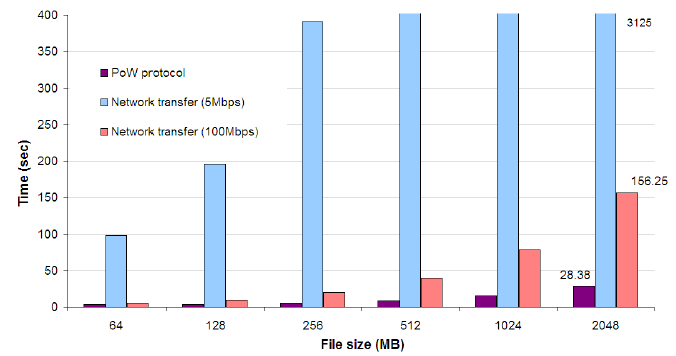
\includegraphics[width=0.8\textwidth]{PoWgraph}
\caption{PoW overall performance\cite{PoW}}
\label{fig:PoWgraph} .
\end{center}
\end{figure}

Protocol is observed in two setups: network with $5Mbps$ and $100Mbps$. The results are following: PoW always consumes less time in $5Mbps$ then transferring the whole file. Once the file grows over the $1GB$ PoW requires 1\%  time of the file transfer. In case of $100Mbps$ network, the protocol has lower bound for file size. For files larger then $64KB$, PoW consumes less time then solution without deduplication . And for files larger then $1GB$, it requires 4\% of time of the whole file transfer. 

\begin{savenotes}
\begin{table}[!htpb]
\centering
\addtolength{\tabcolsep}{3pt}
\begin{tabular}{|L{1cm}|L{4.5cm}|L{4.5cm}|}
\rowcolor{lightblue}
\hline
&Dedup Time  $= T_d$ &File Transfer Time $=T$ \\
\hline
PoW & $\color{red} 3.28T_d+0.7ms$\footnote{For files less then 64Mb: $T_d+0.28T_d+2T_d+0.7ms$}  and $\color{red} 1.28T_d+1.165s$\footnote{For files more then 64Mb: $T_d+0.28T_d+2T_d+0.7ms$ } 
& $\color{red} 0.1T$\footnote{In 5Mbps network and file size more then 1Gb}; $\color{red} 0.4T$ \footnote{In 100Mbps network and file size more then 1Gb}; 
$\color{red} > T$ \footnote{In 5Mpbs for any size of file and In 100Mbps for files larger then 64K}; \\
\hline

\end{tabular}
\caption{PoW 1Time Comparison}
\label{table:paramProbCodes}
\end{table}
\end{savenotes}



\subsection{Solution \# 2}
\label{sub:Soltuion2}
%%%%%%%%%%%%%%%%%%%%%%%%%%%%%%%%%%  Boosting Efficiency and Security in Proof of Ownership for Deduplication - 2012 %%%%%%%%%%%%%%%%%%%%%%%%%%%%%%%%%%
This subsection covers the solution proposed by Di Pietro\cite{DiPietro} in his paper "Boosting Efficiency and Security in Proof of Ownership for Deduplication". The motivation of this work is to improve the efficiency of PoW\cite{PoW} protocol and to avoid the security  assumptions that is hard to verify(refereeing to the concept that the file is taken from some class of distribution and not from arbitrary distribution). The subsection includes the scheme description and efficiency analyses in comparison with PoW\cite{PoW} 

\subsubsection{Setup}
\label{subsub:setup2}


Solution offered by Di Pietro is two party protocol and involves $C$(Client) as a prover and $S$(Server) as a verifier. He names a protocol as s-POW. Once $S$ receives the file for the first time it computes the $n$ number of challenges and stores the file on the disk. To compute the challenges $S$ keeps the hash-map data structure $\Im$. It maps files to the tuples and as a key it uses the hash of the file. Tuple contains four elements: $ptr$ -- the pointer on the file; $res []$ -- an array of generated challenges--called "responses" ($K$ bit strings); $id_c$ -- the highest challenge computed so far ; $id_u$ -- number of challenges used so far.

\begin{figure}[ht] 
\begin{center}
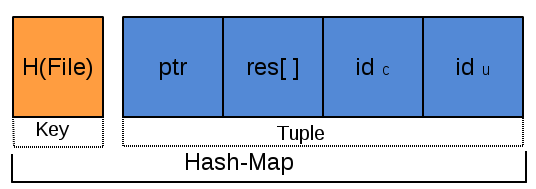
\includegraphics[width=0.8\textwidth]{Di_Pietro_Hash_Map}
\caption{$\Im$ Hash-Map Structure }
\label{fig:Di_Pietro_Hash_Map} .
\end{center}
\end{figure}

The $S$ uses file digest $d$ (hash of the file), $id_c$ index and server's master key as an input for the  pseudo-random generator $F$ to produce random seed $s$. $s$ is an integer and $0 < s < file\_size $. The random seed $s$ serves for calculation of random position in file -- represent as bit vector and is unique for each challenge. At the end  using the random  position and the file as an input, $get-bit$ macros outputs the bit value. Concatenation of such outputs represents the response, which is $K$ bits log and is stored in $res[]$ array. Server computes $n$ number of responses at a time. This approach reduces I/O operations. Computation of responses takes place only, when the client uploads the file, which did not exist on server before or when  all the pre-computed responses are depleted.($id_c$ and $id_u$ control which responses is still valid and how many valid ones are remained.)\\\\
If client $C$ attempts to upload the file already located on server $S$, $S$ challenges the client, sends the random seed $s$ and waits for valid response. Client receives $s$ and use same $get-bit$ macro to produce a $K$ bit length response. If received response is the same as pre-computed one, the client succeeds to convince the server.\\\\
The s-POW protocol has two other modifications, which are designed to improve efficiency and are more convenient in particular cases. In one case the hash function which is used to calculate the key of the hash-map is substitute with calculation of response($K$ bit strings) based on the file and the public seed $S_{pub}$. (This response serves as the key of hash-map) . In second case the file size is used as the key of the hash-map. The second solution is worthy only for large files, as the collision will be extremely high otherwise.

\subsubsection{Security And Efficiency}
\label{subsub:secAndeff2}

To demonstrate the security of s-POW protocol, Di Pietro shows the probability of adversary to convince the verifier and it is assumed that adversary already owns some large part of file. The Probability of adversary to guess the single bit for the $K$ bit length response is: $P(succ_1) = 1-\varepsilon(1-g)$, where $\varepsilon$ is fraction of file that is unknown for attacker and $g$ is the probability to guess unknown bit correctly. To convince the server, the adversary should guess the whole $K$ bit length response, and as guessing each bit from $K$ bit vector are independent events, the probability of convincing server is: $P(succ) = (1-\varepsilon(1-g))^K$. It means that the success probability  of adversary to convince the server depends on $K$, which is possible to tune based the security requirement. E.g. if the requirement is , $P(succ)\leq2^{-k}$, where $k$ is a security parameter, then $K =\lceil \frac{k ln 2}{\varepsilon(1-g)} \rceil $\\\\
Efficiency analyses comprises  the CPU computation, I/O  in bought client and server side and bandwidth. Di Pietro evaluates his proposed schemes(s-POW and s-POW1 \footnote{Modification of s-POW protocol, which uses $K$ bit string  instead of file hash as a key in hash-map}) and compares it with PoW.\footnote{"We have run our implementation of both schemes on a 64-bit RedHat box with an Intel Xeon 2.27GHz CPU, 18 GiB of RAM and an IBM 42D0747 7200 RPM SATA hard disk drive."}\cite{PoW} On client-side both s-POW and s-POW1 schemes are faster then PoW. The complexity up growth of s-POW and PoW schemes are equivalent of file size growth. It is reasonable because in both cases the dominant operation is hashing. While in s-POW1 computation cost becomes  constant for large files. As in the s-POW1 no hashing is used and only random disk access is needed to get required bit. For  visualization it is better to refer  the \hyperref[fig:POWvsPoW]{diagrams} provided by authors:
\begin{figure}[ht] 
\begin{center}
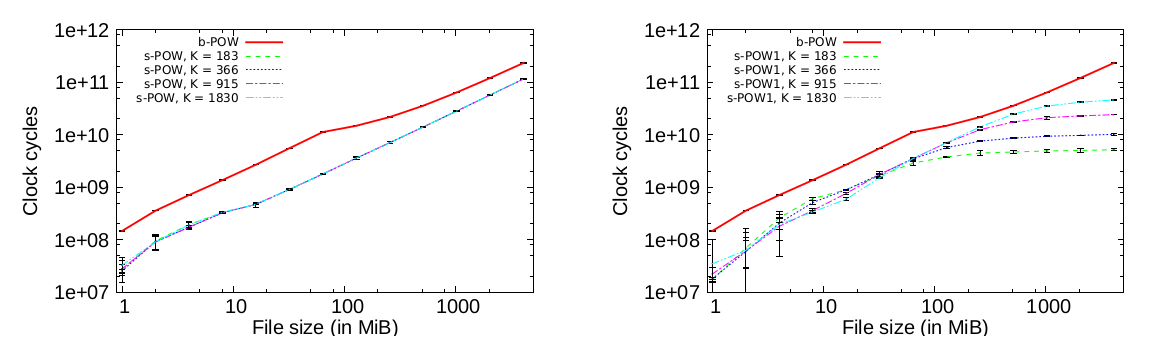
\includegraphics[width=1.0\textwidth]{POWvsPoW}
\caption{Comparison of running time on client-side \cite{DiPietro}}
\label{fig:POWvsPoW} .
\end{center}
\end{figure}

To demonstrate the server-side performance, it is convenient to divide it in two phases: initialization and regular execution. When the file is first uploaded on server-side, that represent initialization phase, all other communication between client and server is the regular execution phase. In initialization phase PoW and s-POW both performs file hashing. It follows with reduction and mixing phase and Merkle-tree calculation in case of  \hyperref[sub:Soltuion1]{PoW} and $n$ challenge computation in s-POW case. In s-POW when all pre-calculated challenges are used, server should pre-calculate them again but this is considered to be a part of regular execution phase. In regular execution phase the  \hyperref[sub:Soltuion1]{PoW}  performs Merkle-tree verification while the s-POW performs only look-up to get the correct tuple and the valid response from $res[]$  array. But in addition to look-up, s-POW needs to recalculate the challenges(responses). Dispite the pre-calculated challenges, which are done in order to decrees the file access, on server side PoW is faster then provided s-POW. It is also important to mention the storage efficiency, PoW need only Merkle-tree root value to store on server side, while s-POW for operation requires storing of the hash-map data structure.  Based on the performed analyses and execution, authors give the \hyperref[table:asymptoticAnalysis]{asymptotic analyses} of schemes. 


\begin{savenotes}
\begin{table}[!htpb]
\centering
\addtolength{\tabcolsep}{3pt}
\begin{tabular}{|L{6cm}|L{2.5cm}|L{2.5cm}|L{2.5cm}|}
\rowcolor{lightblue}
\hline
&PoW&s-POW&s-POW1\\
\hline
Client-side computation&$O(m)hash$ & $O(m)hash$ & $O(k)PRNG\footnote{Pseudorandom number generator}$ \\
\hline
Client-side I/O&$O(m)$&$O(m)$&$O(k)$\\
\hline
Server-side computation (initialization phase)&$O(m) hash$&$O(m) hash$&$O(nk)PRNG$\\
\hline
Server-side computation (regular execution phase)&$O(1)$&$O(nk) PRNG$& $O(nk)PRNG$\\
\hline
Server-side I/O (initialization phase)&$O(m)$&$O(m)$&$O(nk)$\\
\hline
Server-side I/O (regular execution phase)&$0$&$O(nk)$&$O(nk)$\\
\hline
Server-side storage&$O(1)$&$O(nk)$&$O(nk)$\\
\hline
Bandwidth&$O(k\ log\ k)$&$O(k)$&$O(k)$\\
\hline

\end{tabular}
\caption{Asymptotic analyses of schemes.POW,s-POW and s-POW1. $n$ is the number of challenges; $m$ is the file size; $k$ is a security parameter. \cite{DiPietro}}
\label{table:asymptoticAnalysis}
\end{table}
\end{savenotes}



\subsection{Solution \# 3}
\label{sub:Soltuion3}
%%%%%%%%%%%%%%%%%%%%%%%%%%%%%%%%%% Provable Ownership of File in De-duplication Cloud Storage - 2013  %%%%%%%%%%%%%%%%%%%%%%%%%%%%%%%%%%
The subsection reviews the solution offered by Chao Yang in his work "Provable Ownership of File in De-duplication Cloud Storage".\cite{POF} Provable Ownership of File, referred as a POF scheme, is two party protocol and helps the client to prove to the server that it indeed owns the file. The subsection first descripes the scheme, followed by the security and efficiency analyses. To demonstrate the  advantage of their scheme,  authors make comparison with \hyperref[sub:Soltuion1]{PoW} protocol.

\subsubsection{Setup}
\label{subsub:setup3}

POF is a cryptographic protocol that obliges a client to prove to the server that it owns the whole file.The client first sends the hash of the file to the server and if such hash already exist on server side, the POF protocol invokes and the server challenges the client to prove the file possession. The POF consists of two phases: setup and challenge. In setup phase server decomposes the file $F$ in $f$ blocks. It chooses a random number  $R_c$  and generates session key $K_s = h_{sk}(R_c)$ (where $sk$ is pre-shared symmetric key) and two random seeds $S_1$ and $S_2$. Those random seeds are used in challenge phase to choose the blocks of the  file. Server provides the client with random number $R_c$, in order to generate the same session key $K_s$. Client generates the $K_s$ session key and  send back to server the $h_{K_s}(R_c, TS)||TS$ (where $TS$ is the current timestamp) value to confirm the generation of session key.  The session key $K_s$ is keep in secret and is used in challenge phases, while the $R_c$ could be deleted.\\\\
In challenge phase server sends the $c$ number of blocks($1 \leqslant c \leqslant f $) and two random seeds $S_1,S_2$ to the client. Random seeds $S_1$ and $S_2$ are used to produce block indices $i_\tau$ and dynamic coefficient $\delta_\tau$  where ($1 \leqslant \tau \leqslant c$). Client decomposes the whole  file in $f$ block $F=(b_1,b_2,b_3,..b_f)$ and computes the proof as hash of concatenation of the hashes of choose block and dynamic coefficients.  $V' = h_{K_ss}(h_{K_s}(b_{i_1},\delta_1)||h_{K_s}(b_{i_2},\delta_2)|| ...||h_{K_s}(b_{i_\tau},\delta_\tau))$. Client sends to the server the generated proof $V'$, server makes the same calculation, but uses the original file and generates the $V$ proof. If $V'=V$ the server is convinced that the client  owns the file. 
 


\subsubsection{Security And Efficiency}
\label{subsub:secAndeff3}


The POF has three major security requirement. First -- randomness of indices for the blocks of the file. Second -- the original file  must be involved for calculation the proof. And third -- the calculated proof should be different for different times. When all these three security requirement holds the scheme resistants to cheating is as high as the resistants of collision attack of the hash function used in POF. The authors provide the proof of the following theorem: "For the proposed POF scheme, the complexity for cheating of the ownership verification is at least as difficult as performing strong collision attack of the hash function"\\\\
To demonstrate the efficiency of the POF scheme, it is compared with \hyperref[sub:Soltuion1]{PoW}. The authors execute both schemes in the same setup\footnote{The experiments were conducted on an Intel 3.0GHz Intel Core 2 Duo system with 64KB cache, 1333MHz EPCI bus, and 2048MB of RAM. The system runs Ubuntu10.04, kernel version 2.6.34. We used C++ for the implementation. We also used the SHA256 from Crypto++ version 0.9.8b\cite{crypto}. The files are stored on an ext4 file system on a Seagate Barracuda 7200.7 (ST23250310AS) 250GB Ultra
ATA/100 drive.} and demonstrate the results for each of them in $milliseconds$. Two protocols computation time is decomposed in three parts: client, server and network computation time.\\\\ 
Client computation time is covered in details. For POF protocol it includes, time to read randomly chosen parts of original file, key derivation time and time to compute the proof. While PoW for simplicity, includes just whole file reading and Merkle-tree calculation time on original file.(reducing and mixing phases are omitted) And even in this scenario POF is more time efficient on client side. In POF file's portions reading time increases as file size increase, but the time for proof computation could stay the same and does not depend on file size. For PoW -- the whole file reading time and Merkle-tree computation time, both increase as file size grows. Based on results,(see \hyperref[Appendix 1] {Appendix 1})  we can demonstrate  the difference in client time computation (in average), between POF and PoW schemes. The schemes had run on different size of files and the file size was doubling each time. The starting size was $0.015625MB$ and it had increased till $1024$MB. We can see that the file size was increased 65536 times. As file size was growing the time consumption was changing. In case of POF  for the disk reading , the time was increased approximately $37$ times and key derivation and  proof computation time was remained mostly constant(around $0.62 ms$). So the total time was increased $8$ times (at stating point the total time was $0.77$ and at the ending point -- $6.15 ms$). In case of PoW -- disk reading was increased $28684$ times and Merkle-tree computation approximately $40955$ times, overall $39296$ time for total time. (at stating point the total time was $0.66$ and at the ending point -- $25926.39 ms$). \\\\
Server side computation time is considered to be same or less then client side computation for POF. In case of PoW it is to check the Merkle-tree authentication signature, which is not time consuming. Network transmitting time, is the time required to transfer the data generated by protocols. In the given setup the data generated for both protocols was less then $1KB$. The server and network times both are negligible and based on the client computation time it was demonstrated that, the POF is more efficient then PoW.

\subsection{Solution \# 4}
\label{sub:Soltuion4}
%%%%%%%%%%%%%%%%%%%%%%%%%%%%%%%%%%%  Leakage-Resilient Client-side Deduplication of Encrypted Data in Cloud Storage - May 8,2013 %%%%%%%%%%%%%%%%%%%%%%%%%%%%%%%%%%

The subsection covers solution offered by Jia Xu and his colleagues in the paper work "Weak Leakage-Resilient Client-side Deduplication of Encrypted Data in Cloud Storage".\cite{Leakage-Resilient} In previous solutions reviewed in this work, the server is considered as a honest player and effort is directed to prevent malicious clients. While this paper address both client and server side threats. Paper underlines the importance of confidentiality of user's sensitive data. It claims that, the remote storage provider should not have access to the users sensitive information and proposes the solution of Proof of Work protocol over the encrypted files on client side. Jia Xu expends the security restriction of Halevi's \hyperref[sub:Soltuion1]{PoW}  protocol, from specific class of file distribution to arbitrary file distribution. But on the other hand it restricts the data leakage size and security holds if the leakage takes place only before the protocol starts, while in PoW leakage could happen any time, but not the during protocol communication.\\\\
Using encryption on client side delivers confidentiality of sensitive information but, on the other hand it rises the risk of \textit{Poison Attack}, also known as \textit{Target Collision attack}.\cite{PoisonAttac} When encrypted file is uploaded on server side, server is not able to check consistency between file and meta-data (e.g. hash of the file). This feature opens possibility to attacker to substituted the encrypted file with the same size malicious one. And if later the owner of the file retrieves it, she gets poisoned file not the original one. Solution demonstrated in this subsection, takes into consideration these type of threats and  offers solid security over some restricted leakage conditions.


\subsubsection{Setup}
\label{subsub:setup4}

The Weak Leakage-Resilient Client-side Deduplication scheme, is refereed as $CSD$ shortly and is represented with four probabilistic polynomial-time algorithms $E, D, P, V$ .  $E$ is an encryption algorithm: $E(F,1^\lambda) 	\rightarrow (\tau, C_0, C_1)$, where $F$ is file, $\lambda$ is security parameter, $\tau$ encryption key and $C_0\ and\ C_1$ are cipher-texts: $C_0$ -- encrypted key and $C_1$ -- encrypted file. $D(\tau,C_1) \rightarrow F $ -- decodes $C_1$ cipher. $P(F) \rightarrow y_0,\  y_0 \in \{\tau,\perp\} $ -- prover algorithm , which interacts with verifier algorithm and outputs the encryption key $\tau$. $V(C_0) \rightarrow (y_1,y_2),\ y_1 \in \{Accept; Rejectg\}\ and\ y_2 \in \{hash(C_1),\perp \}$ -- verifier algorithm, which interacts with prover algorithm.\\\\
The $CSD$ protocol involves the client and the server. When a client uploads the file first time on the server, it generates the random AES\cite{AES} key $\tau$ and two ciphers: $C_F$ and $C_\tau$. Where $C_F$ is an encrypted file, using AES encryption and generated  key $\tau$  and is almost as large as original file. While  $C_\tau$ is the encrypted random key $\tau$ generated by client, using some custom encryption method and the file $F$ as a key. And the size of $C_\tau$ is small number -- upper bounded by $|\tau|$. After the key and ciphers are generated, client sends hash value of original file $F$, together with two cipher $C_F$ and $C_\tau$.  Server receives the data form client, stores the encrypted file $C_F$ in secondary storage(large but slow storage). While meta-data of encrypted file is stored in primary storage and is represented as key-value pair entry in the lookup database: $(key = hash(F); value = (hash(C_F), C_\tau))$ , where $hash(C_F)$ is calculated by server and $hash(F)$ and $C_\tau$ is received form client.\\\\
If client tries to upload the file -- already located on the server side, it first sends the $hash(F)$ to the server.  Based on the received $hash(F)$, the server identities  the tuple $(hash(C_F),C_\tau)$ in the lookup database. It retrieves the $C_\tau$ value and sends back to client. If the client indeed owns the file, she can decrypt the cipher $C_\tau$ using the file as a decryption key and retrieve the ASE key $\tau$. After obtaining the AES key $\tau$, client encrypts the original file, computes the hash of it and sends the $hash(C_F)$ as a proof to the server. Server compares the received $hash(C_F)$ hash value, with the one kept in its lookup database. If the values are equal then the client gains the access to the file, otherwise access is forbidden. After client is identified as honest, she can remove the original file and keep only the ASE key $\tau$, which she will use later for decrypting the downloaded file.\\\\




\subsubsection{Security And Efficiency}
\label{subsub:secAndeff4}

To demonstrate the security of the $CSD$ scheme, authors use the game-based security proof. The security definition states that, adversary can not learn anything new about the a single bit of the file( thereof about the file in  whole), from client-side deduplication process, besides the side channel leakage. Security game $G^{CSD}_A$ between challenger and PPT(Probabilistic Polynomial Time) $A$ adversary consists of two learning and two guessing phases. In first learning phase, adversary receives the output of some PPT function $y$ from the challenger. $y < (\varepsilon_0 - \varepsilon_1)$ , where  $\varepsilon_0$ is a minimum min-entorpy of the file and  $(\varepsilon_0 - \varepsilon_1)$ -- is a max length of bits adversary is allowed to learn about the file. For it's part $\varepsilon_0>\varepsilon_1  \geq\lambda$, where $\lambda$ is a security parameter. Adversary chooses the $v$ indices ($i_1, ...i_v$)  and the challenger chooses the subsequence $\alpha \in \{0,1\}^v$  of the file, such that the each bit chosen based on $v$ indices from that subsequence $\alpha$ corresponds the bit from the file $F$ also chosen based those indices. The challenger chooses the bit  $b \in \{0,1\}$ and sets $\alpha_b=\alpha$ and $\alpha_{1-b}  \in_R \{0,1\}^v$ and sends those $\alpha_0$ and $\alpha_1$ to the adversary. It is followed with the first guessing phase, where an other extractor $A_*$ produces the guess of $b$ bit, $b_{A_*} \in \{0,1\}$. In the second guess phase the adversary tries to guess the $b$ bit, $b_A \in \{0,1\}$.\\\\
The $CSD$ is secure in $(\varepsilon_0, \varepsilon_1)$ if the probability of guessing $b$ single bit by extractor $A_*$ plus some negligible in security parameter $negl(\lambda)$, is grater or equal then probability of adversary $A$ guessing the same $b$ bit: $Pr[b_A=b]\leq Pr[b_{A_*}=b]+negl(\lambda)$. Authors construct the secure $CSM$ in the paper and have provide the proof of the security statement in their work.\\\\
The $CSD$ scheme efficiency is measured based on running the prover $P$ and the verifier $V$ interactive algorithms.\footnote{"The test machine is a laptop computer, which is equipped
with a 2.5GHz Intel Core 2 Duo mobile CPU (model T9300), a 3GB PC2700-800MHZ RAM and a 7200RPM hard disk. The test machine runs 32 bits version of Gentoo Linux OS with kernel 3.1.10. The file system is EXT4 with 4KB page siz" \cite{Leakage-Resilient}}It is compared with the running time of transferring files without deduplication or encryption. The \hyperref[fig:CSD]{graph} provided by authors shows, that it is more efficient to use $CSD$ scheme for secure deduplication rather then avoid it at all and transfer whole files via network.\\\\
\begin{figure}[ht] 
\begin{center}
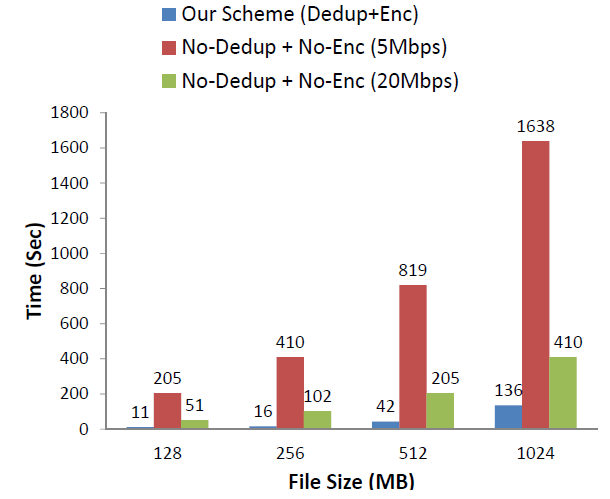
\includegraphics[height=310pt,width=400pt]{CSD}
\caption{$CSD$ efficiency graph \cite{Leakage-Resilient}}
\label{fig:CSD} .
\end{center}
\end{figure}

\pagebreak

\subsection{Solution \# 5}
\label{sub:Soltuion5}
%%%%%%%%%%%%%%%%%%%%%%%%%%%%%%%%%%  A Secure Client Side Deduplication Scheme in Cloud Storage Environments - 2014 %%%%%%%%%%%%%%%%%%%%%%%%%%%%%%%%%%

The subsection reviews the solution offered by Nesrine Kaaniche and Maryline Laurent in their paper work "A Secure Client Side Deduplication Scheme in Cloud Storage Environments".\cite{Kaaniche} Like the last solution, it addresses both the malicious clients and the curious-server issues. It provides the means to control the integrity of both players, neither server no client gets fooled. In addition it address the private file shearing issues. The subsection first covers how the solution operates and provides security and efficiency analyses later.

\subsubsection{Setup}
\label{subsub:setup5}


The security scheme is implemented on OpenStack Swift \footnote{The open-source cloud storage project - \url{https://www.swiftstack.com/product/openstack-swift}, last seen October 4, 2016} platform and is based on  convergent encryption concept\cite{CovergentEnc}, but for identification it uses Merkle-tree signature. The authors give a clear and simple \hyperref[fig:ConvMT]{scheme} of cloud storage architecture.
\begin{figure}[ht] 
\begin{center}
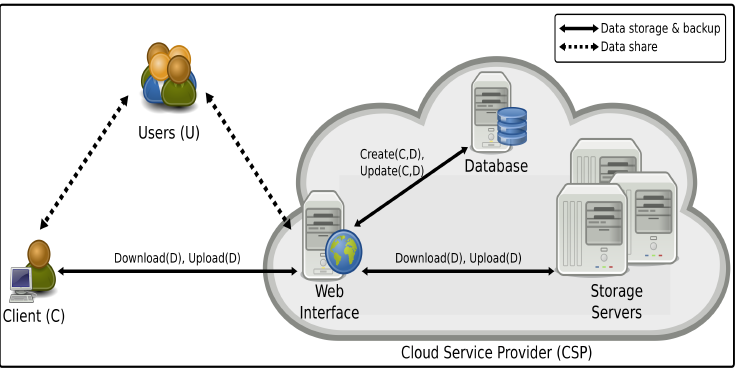
\includegraphics[height=210pt,width=400pt]{ConvMT}
\caption{Client uploads and stores the data on server and Users are allowed to access (depend on their access rights) the content of stored data \cite{Kaaniche}}
\label{fig:ConvMT} .
\end{center}
\end{figure}
When data owner desires to outsource the file $F$ on the remote server, he first encrypts it, and uses the file content hash $K_F$ as an encryption key. He builds the Merkle-tree on the encrypted file and  uses the root value $MT_F$ as the file identifier, which is unique on the remote storage. Client sends the $MT_F$ identifier\footnote{The client also adds nonce $n$ to the identifier to avoid a replay attack} to the server and checks whether the file already is located on the server or not. The server checks in the database and if the received identifier does not matches, asks client to upload the file. The client in his turn, sends the encrypted file and the encryption key $K_F$ -- encrypted by the public keys of the authorized users (users with whom client desires to share the file). Later the encrypted key $K_F$ is included in the file meta-data. After the server stores the file, it sends the acknowledgement message to client, which includes the stored file's URI(Uniform Resource Identifier).\footnote{The solution is implement on Swift, which is an object store, so each file could be reached by URI}\\\\
If the file is already located on the server, then the server sends to the client some number of random indecies of Merkle-tree leaves. The client calculates the sibling paths of chosen leaves  and sends (leaves together with sibling paths) as proof of ownership to the server. The server validates the received proof and if it holds, it sends acknowledgment on storing the file and the URI of requested file to the client. Otherwise, client is failed to access the file.\\\\
When client desires to access the outsourced data he owns -- he sends the file URI to the server. The server, checks in the database, whether the client owns the file. If the client is the owner of the requested file, server sends encrypted file to the client. After receiving the file, client first extracts the file meta-data(i.e. encrypted $K_F$ encryption key), decodes the encrypted $K_F$ key with own private key and use $K_F$ to decode extracted file.\\\\




\subsubsection{Security And Efficiency}
\label{subsub:secAndeff5}
Authors offered very brief overview of security, without any game-based or simulation-based security proof. They address three main issues in their scheme: Data confidentiality, privacy and access control.  When client wants to store new data to the remote storage, he calculates the Merkle-tree  over the encrypted file and sends the root value together with nonce $n$. Nonce  prevents from replay attacks\footnote{"Replay attacks are the network attacks in which an attacker spies the conversation between the sender and receiver and takes the authenticated information"}(stilling the identifier), while transferring the data. But if the adversary still will be able to obtain the identifier (root value of the Merkle-tree), he is required to proof the ownership of the file and this proof is based on Merkle-tree lemma \cite{MerkleLemma} and prevents malicious client to access the confidential data. Scheme also prevents curios  servers to reach  the users' private data and built users' profile. The server is not able to access the data, because it is encrypted and the encryption key is secured with asymmetric encryption. Access control is managed by embedding the symmetric encryption key $K_F$ encrypted by public keys of the users who are authorized to access the file.\\\\
To evaluate the performance of the solution, authors implement the OpenStack swift framework and integrate it with their own scheme for security.\footnote{"For our tests, we used 1000 samples in order to get our average durations. In addition, we conducted our experiments on an Intel core 2 duo, started on single mode,where each core relies on 800 MHz clock frequency (CPU).\cite{CovergentEnc}"} The scheme's performance time is decomposed in two parts: Client and Server computation time. The client computation time is consist of the data encryption/decryption time and data upload/download time. For encryption/decryption of file the scheme uses symmetric AES(Advanced Encryption Standard) in CBC(Cipher Block Chaining) mode.
The authors examine the performance of file encryption/decryption using different key sizes(key size = $128, 192\ or\ 256 bits$) of AES encryption and different file input sizes (file size = $k * 10^5$ where $k \in \{ 1,2,..10\}$ ).  The results  exposes -- the computation time is dependent on a key size and a file size and as they are increasing the time of computation increases as well. The encryption/decryption time for the smallest key($128 bits$) and the smallest input file size($0.1 MB$) is 1 ms, while with the largest key size and input file size (key size = $256 bits$, file size = $1MB$) is less then 12 ms.  The authors examine the upload/download time and the results shows -- uploading time is greater then downloading time. Also time remains constant for small files (file size < $5*10^4$ bits), while for  larger files it depends on file size and time increase as the file size increases. To compare the cryptographic operations to the file transfer operation on client-side, it is easy to see that cryptographic operations are consuming much less time, then file upload/download. And the comparisons that is given in the paper \cite{CovergentEnc} claims, that encrypting of the  $0.8 MB$  size file takes $0.1ms$, while uploading it takes $10s$, which means the encryption operation is 1\% of uploading operation. For securing the AES encryption key, the scheme uses ECC (Elliptic Curve Cryptography).\cite{ECC}  Unfortunate the paper\cite{CovergentEnc} does not covers the server time consumption and there is no any comparisons with other schemes. 


\subsection{Solution \# 6}
\label{sub:Soltuion6}
%%%%%%%%%%%%%%%%%%%%%%%%%%%%%%%%%% A Tunable Proof of Ownership Scheme for Deduplication Using Bloom Filters - 2014 %%%%%%%%%%%%%%%%%%%%%%%%%%%%%%%%%%
This subsection is dedicated to a paper work "A Tunable Proof of Ownership Scheme for Deduplication Using Bloom Filters".\cite{BF} The paper offers  the data ownership proof scheme based on Bloom Filter.\cite{BF-Original} The bloom filter is a time and space efficient data structure. It serves to identify, whether the element is  the member of the set or not. The issue with this data structure -- it has false positives. The element which does not belongs to the set, could be considered as the member, but never vice-versa. Bloom filter allocates $s$ bits length vector (all bits set to $0$) and uses $n$ number of different evenly distributed hash factions. To add the element in bloom filter, the element is hashed with the $n$ different hash functions. The results of hashes is the indecies in the $s$ bits length vector and in those indecies bits are set to $1$. To check if the particular element belongs the set, it must be hashed using the $n$ different hash functions to produce the indecies. After the indecies are produced, the vector is examined in those indecies and if all the bits are set to $1$, then the  element belongs the set.


\subsubsection{Setup}
\label{subsub:setup6}
The Proof of Ownership Scheme for Deduplication Using Bloom Filters, also referred as bf-POW is the two party protocol. It represents an interaction between $C$ as a client and the $S$ as a server. There are two scenarios, first when uploading the file first time on the server and second trying to upload the file already located on the server. In the first scenario, client  sends the hash of the file  $h_f$  to the server. The server identifies that the file is unique, based on the fingerprint $h_f$ and asks the client to upload the whole file $f$ and initializes all the required data structures, including bloom filter. After receiving the file $f$, server divides it into the equal size chunks, then computes the tokens, using some hash function: $H:\{0,1\}^B\to\{0,1\}^l$, where the $B$ is a chunk size and $l$ is a token size. And finally the indecies are generated form token using some pseudo random function, $PRF: \{0,1\}^l \to \{0,1\}^{n}$ where $n$ is a positive  integer. Those indecies are inserted in the bloom filter $BF$ data structure. The server keeps the associative array $A$, which use the hash of the file $h_k$ as a key and the tuple $\{f,BF,AL\}$ as a value. In the tuple the $f$ is the content of the file, $BF$ represents the bits in the bloom filter and the $AL$ is the list of the client identifiers $id(C)$, who are owning the file. After the file is uploaded first time on the server , the entry is added to the array $A$.\\\\
In the second scenario, when the file is already located on the server, there is no need to upload the file, instead the client must proof that he indeed owns it. The server initializes the array $pos$, which holds the randomly chosen chunks' indecies and $J$ is the length of the $pos$ array. The server sends $pos$ array to the client and waits for the tokens generated based on $pos$ array. The client performs the same operation as the server, in order to generate the tokens and creates the array $res$ which holds the generated tokens.  $res[i]\gets H(f[pos[i]])$ where $ 0 \leq i < J$ and $J$ is the number of randomly chosen indecies. The client sends $res$ array to server and the server generates the indeces based the $PRF$ and the  $res$ array and checks whether each output $PRF$ belongs to bloom filter or not. If all outputs belongs to bloom filter then the client is considered as the file owner and the $id(C)$ is added to the $A[h_f].AL$ list. Otherwise the client fails to proof the file ownership. Later when client request to download the file , the server will check, if the $id(C) \in A[h_f].AL$



\subsubsection{Security And Efficiency}
\label{subsub:secAndeff6}


To demonstrate the security of the bf-POW scheme, authors evaluate a probability of the adversary $\bar{C}$ convincing the server without owning the file. The adversary is allowed to communicate with file owners and receive some information about the file (but not during while the protocol takes place). The probability that adversary knows the $B$ bits long randomly chosen chunk of the file is $p$. And the probability to guess the randomly chosen byte is $g$. In order to pass the proof the adversary $\bar{C}$ should provide $J$ tokens, based on randomly chosen $J$ chunks by the server. And those tokens used as seeds of $PRF$ should produce the indecies which will belong to the bloom filter for the given file $f$. In order to succeed there are two options. First $\bar{C}$ should produce the correct token and the second -- occurrence of false positive when checking for bloom filter membership. The probability of false positive in bloom filter is -- $p_f$. The $p_f$ depends on the size of the bloom filter and the number of hash functions.\footnote{If $J$ is a total number of elements that could be inserted in the bloom filter and $p_f$ is the probability of false positives, then the size of bloom filter is $s=\lceil - \frac {N\ ln\ p_f} {(ln2)^2}\rceil$ and the number of independent hash functions is $n=\lceil\frac{s} {N}ln2\rceil$} The probability to produce one randomly chosen token from the $J$ tokens correctly is $P(in_i)=P(tok_i)+p_f*P(\bar{tok_i}) \  (1)$ where $in_i$ and $tok_i$ are both events: $in_i$ --  i-th generated token, is a seed of the index which is the member of bloom filter; $tok_i$ -- adversary generates token correctly. In its part probability of event $tok_i$ is decomposed as the probability of knowing the chunk and probability of guessing it. The $p$ is the probability that the adversary knows the $i$-th chunk.  If adversary knows the $i$-th chunk, it means that he is able to compute the $i$-th token correctly. If he does not know, he should guess. Probability of guessing $B$ bits long chunk is lower, then probability of guessing $l$ bit token directly, $g^B << 0.5^l$. From adversary perspective better to guess directly a chunk. And $P(tok_i)=p+(1-p)*0.5^l \  (2) $ In order to succeed adversary needs to produce $J$ number of tokens form randomly chosen chunks. To compute the probability of success, we use these two formulas : $(1)$ and $(2)$\\\\
$P(succ)=P(in_i)^J=(P(tok_i)+p_fP(tok_i))^J=(p+(1-p)*0.5^l + p_f*(p+(1-p)*0.5^l))^J=(p+(1-p)*0.5^l)+p_f(1-p)(1-0.5^l)^J=(p+(1-p)(0.5^l)+p_f(1-0.5^l))^J$\\\\
We can see that the probability   of success dependents on $J$. And it is possible to choose $J$ in such a way that the $P(succ) \leq 2^{-k}$ , which is negligible in the security parameter $k$.\\\\
Authors provide the asymmetric analyses and the results of the experiments of bf-POW, in comparison with \hyperref[sub:Soltuion1]{POW} and \hyperref[sub:Soltuion2]{s-POW} schemes. In bf-POW each time the client tries to upload the file, he hashes it. Also the client is required to calculate the tokens, meaning the $J$ times hashing operation over the $l$ length chunks. On server side there are two phases, with different computation complexity in each phase. In initialization phase (when the file is uploaded first time on server side) the dominant cost is the hashing operations used to insert elements in bloom filter. As there are $n$ different functions, it requires $n$ hashing operations. Also in initialization phase server should load the whole file into the memory, while in execution phases (when the file is already located on the server) the server needs only bloom filter to be loaded in the memory, and the indecies are generated by hashing the tokens received from client.(res[] array). In terms of bandwidth efficiency, bf-POW generates $J$ tokens. (the client sends tokens to the server in order to proof ownership). 
The complexity of the schemes is represented in big-O notation, is provided by authors in the following  \hyperref[table:asymptoticAnalysisBF-POW]{table} : 

\begin{savenotes}
\begin{table}[!htpb]
\centering
\addtolength{\tabcolsep}{3pt}
\begin{tabular}{|L{5cm}|L{2.5cm}|L{2.5cm}|L{3.5cm}|}
\rowcolor{lightblue}
\hline
&PoW&s-POW&bf-POW\\
\hline
Client computation&$O(F)hash$ & $O(F)hash$ & $O(F)hash$ \\
\hline
Client I/O&$O(F)$&$O(F)$&$O(F)$\\
\hline
Server init computation &$O(F) hash$&$O(F) hash$&$O(F)hash$\\
\hline
Server regular computation &$O(1)$&$O(nk) PRF$& $O(\frac{l*k*(log1/p_f)}{p_f})hash$\\
\hline
Server init I/O &$O(F)$&$O(F)$&$O(F)$\\
\hline
Server regular I/O &$O(0)$&$O(nk)$&$O(0)$\\
\hline
Server memory usage&$O(1)$&$O(nk)$&$O(\frac{log(1/p_f)}{l})$\\
\hline
Bandwidth&$O(k\ log\ k)$&$O(k)$&$O(\frac{lk}{p_f})$\\
\hline

\end{tabular}
\caption{Asymptotic analyses of schemes:POW,s-POW and bf-POW. $F$ is the file size; $k$ is a security parameter; $n$ is number of challenges in s-POW;  $l$ is a $PRF$ output size; $p_f$ is a probability of false positive in BF \cite{BF}}
\label{table:asymptoticAnalysisBF-POW}
\end{table}
\end{savenotes}
 
The authors have implement \hyperref[sub:Soltuion1]{POW}, \hyperref[sub:Soltuion2]{s-POW} and their bf-POW schemes, in order to compare the time performance results to each other. \footnote{"The benchmarks are run on an Intel Xeon 2.27GHz CPU with 18 GiB of RAM running RHEL Server release Santiago (6.1). The input fles contain random data, and their size ranges from 1 MiB to 4 GiB, with the size doubled at each step."} The results show that in bf-POW the better performance is dependent on the size of token, which in its part also decries bandwidth consumption. Smaller tokens influence the size of bloom filter and increase it in order to keep the security in place.(decries the probability of false positives.)  In the worst case bloom filters require  $2MB$ additional storage per file. Bf-POW is always faster then s-POW scheme on server side and is the fastest  among those three on server side for specific $p$ ($p$ is the probability that adversary knows the randomly chosen chunk of the file). On client side, bf-POW is faster then POW and is a litter slower then s-POW.
 
 


\subsection{Solution \# 7}
\label{sub:Soltuion7}
%%%%%%%%%%%%%%%%%%%%%%%%%% An efficient confidentiality-preserving Proof of Ownership for Deduplication -2014  %%%%%%%%%%%%%%%%%%%%%%%%%
"An efficient confidentiality-preserving Proof of Ownership for Deduplication" paper work\cite{ce-POW},  is the last solution, refereed as the ce-POW, covered in this thesis. The ce-POW scheme address the privacy and confidentiality issues in remote storage and considers both malicious client and honest-but-curios server as an adversary. It uses the mix of convergent encryption and proof of ownership protocol, and ensures to avoid poison attack, which is considered to be the drawback of original solution of convergent encryption. Like the previous subsections, this also  covers setup of the scheme, describes how it operates and analyses its security and efficiency. 



\subsubsection{Setup}
\label{subsub:setup7}
The ce-POW is two party protocol, involving client $C$ as a prover (each client $C$ has its' own identifier $id(C)$) and the server $S$ as a verifier. The protocol has two phases: Initialization  and Challenge. When client uploads the file first time on the server, it is considered as an initialization phase. Client sends the file size to the server, in order to receive the number of chunks to dived the file. After the client obtains the number $N$, he divides the file $f$ into $N$ chunks, encrypts each of them using convergent encryption\footnote{CE -- convergent Encryption uses the content hash as an encryption key, in this case it use $H_2:\{0,1\}^B\rightarrow\{0,1\}^l$}, hashes each encrypted chunk $token[i]=H_2(E_{H_2(f[i])f[i]})$ using the $H_2:\{0,1\}^B\rightarrow\{0,1\}^l$ where $B$ is the chunk size and the $l$ is a token size and $f[i]$ is the $i$-th chunk of the file. And based on array of $token[]$ generates the fingerprint $h_c$, using the hash function $H_1:\{0,1\}^*\rightarrow\{0,1\}^n$. The client sends to the server all the encrypted chunks together with the fingerprint $h_c$. After server receives the data from the client, based on encrypted chunks it calculates the $h_c$ in order to avoid the poison attack. If the calculate fingerprint is the same as the received one from the client, the server inserts the entry in the associative array $A$, which exist on server side and takes part in challenge phase.  The  associative array $A$ uses the fingerprint $h_c$ as a key and  $\{ENC, CH, RES, AL\}$ tuple as a value, where $A[h_c].ENC$ stores the encrypted chunks; $A[h_c].CH$ -- 10 000 challenges, each represents the $J$ number of chunk indecies; $A[h_c].RES$ -- expected responses on the challenges and   $A[h_c].AL$ keeps the list of legitimate file owners.\\\\
If client tries to upload the file already located on the server, it is the challenge phase and client sends the $h_c$ and the server identifies that the file $f$, with the fingerprint $h_c$ already located on the disk and there is no need to upload it.(If there is no entry in the associative array $A$, with the key $h_c$, the initialization phase stars.) Instead the server challenge the client to prove the file ownership. The server picks the first unused challenge --  $pos[]$ which is $J$ size in order to hold the randomly chosen $J$ chunks' indecies and sends it to the client. The client picks the indecies form the $pos[]$  array, calculates the $tokens$ based on those indecies and generates the $res[]$ array, which holds $i$-th token on $i$-th  position. The client sends the array $res[]$ to the server and server compares  pre-calculate responses  $A[h_c].RES[i]$. If the match is found then the client is added in the list of file owner $id().AL$, otherwise the proof of ownership is failed.

\subsubsection{Security And Efficiency}
\label{subsub:secAndeff7}
The security requirement of the ce-POW, claims that the scheme is secure if the probability of the adversary convincing the server is negligible in security parameter $k$ , when the adversary does not owns the part of the file, which is larger then some predefined threshold $S_{min}$.The adversary is allowed to communicate with file owners and receive some information about the file (but only before protocol starts). The probability that adversary knows the $B$ bits of randomly chosen chunk of the file is $p$. And the probability to guess the randomly chosen byte is $g$. In order to pass the proof the adversary $\bar{C}$ should provide $J$ tokens, based on randomly chosen $J$ chunks by the server. And the probability of success is:\\\\
$P(succ) = P(tok_i)^J\ (1)$, where $tok_i$ is an event that  adversary generates $i$-th token correctly.\\\\
The probability of event $tok_i$ is decomposed as the probability of knowing the chunk and probability of guessing it. The $p$ is the probability that the adversary knows the $i$-th chunk.  If adversary knows the $i$-th chunk, it means that he is able to compute the $i$-th token correctly. If he does not know, he should guess. Probability of guessing $B$ bits long chunk is lower, then probability of guessing $l$ bit token directly, $g^B << 0.5^l$($g^B$ -- probability of guessing $B$ bits;$0.5^1$ -- probability of guessing l bit token). From adversary perspective better to guess directly a chunk. Then the probability of guessing the $i$-th token correctly is:  $P(tok_i)=p+(1-p)*0.5^l\ (2)$.Substitute $P(tok_i)$ in  formula $(1)$ with  formula $(2)$: $P(succ) = P(tok_i)^J = (p+(1-p)*0.5^l)^J$. We can see that the probability of success dependents on $J$. And it is possible to choose $J$ in such a way that the $P(succ) \leq 2^{-k}$ , which is negligible in the security parameter $k$.\\\\
To demonstrate the efficiency of the the ce-POW scheme, authors provide the asymptotic  analyses and experimental results of the implementation. The ce-POW is compared with \hyperref[sub:Soltuion2]{s-POW} and \hyperref[sub:Soltuion6]{bf-POW} solutions. In client side ce-POW requires encryption and computation of two hashes, while bf-POW computes the hash of the whole file each time it makes a request to the server. On server side  in initialization phase, the bf-POW make $n$ number of hash operations in order to insert the element in bloom filter. For ce-POW the  cost is  two hashing operations. The bandwidth consumption for ce-POW is $J$ \footnote{ the implementation has 4 different size of tokens $16, 64, 256\ and\  1024\ bits$} tokens that, a client sends to server in order to prove the data ownership. The number of tokens increases as the security parameter $k$ is increasing. The bf-POW has  similar  bandwidth consumption, in difference that the number of $J$ tokens could be  shortened in exchange of rising the false positives in bloom filter. While the s-POW needs only to transfer $K$ bits of randomly chosen from file. Authors provide asymptotic analyses in the \hyperref[table:asymptoticAnalysisCE-POW]{table}  :


\begin{savenotes}
\begin{table}[!htpb]
\centering
\addtolength{\tabcolsep}{3pt}
\begin{tabular}{|L{4cm}|L{4cm}|L{2.5cm}|L{3.5cm}|}
\rowcolor{lightblue}
\hline
&ce-PoW&s-POW&bf-POW\\
\hline
Client computation&$O(B)*CE*hash*hash$ & $O(F)hash$ & $O(F)hash$ \\
\hline
Client I/O&$O(F)$&$O(F)$&$O(F)$\\
\hline
Server init computation &$O(B)*hash*hash$&$O(F) hash$&$O(F)hash$\\
\hline
Server regular computation &$O(n * l *k)*PRNG$&$O(nk) PRF$& $O(\frac{l*k*(log1/p_f)}{p_f})hash$\\
\hline
Server init I/O &$O(F)$&$O(F)$&$O(F)$\\
\hline
Server regular I/O &$O(0)$&$O(nk)$&$O(0)$\\
\hline
Server memory usage&$O(n * l *k)$&$O(nk)$&$O(\frac{log(1/p_f)}{l})$\\
\hline
Bandwidth&$O(l *k)$&$O(k)$&$O(\frac{lk}{p_f})$\\
\hline
\end{tabular}
\caption{Asymptotic analyses of schemes: ce-POW,s-POW and bf-POW. $F$ is the file size; $k$ is a security parameter; $n$ is number of challenges in s-POW;  $l$ is a token size; $p_f$ is a probability of false positive in BF \cite{ce-POW}}
\label{table:asymptoticAnalysisCE-POW}
\end{table}
\end{savenotes}

Three schemes ce-POW, s-POW and bf-POW was implement, in order to compare their performance results. \footnote{"The experiments have been performed on a AMD Athlon(tm) II x2 220
processor with 4GB of RAM. Input fles have been randomly generated and their sizes range from 4MB to 2GB doubling the size at each step."} For ce-POW implementation the parrameters was chosen in following way: security parameter $k$ was set to $66$, threshold of leakage $S_{min} = 64MB$, tokens size $l \in \{16, 64, 256,1024\} $, probability of adversary knowing the  chunk of file $p \in \{0.5; 0.75; 0.9; 0.95\}$ and number of requested challenges $J \in \{91, 182, 457, 914\}$.
The results shows that in initialization phase on server side the fastest scheme is bf-POW. In bf-POW the server initializes and inserts the elements in bloom filter. To insert the element in bloom filter server divides the file in chunks, computes the tokens form chunks which is hashing operation and then computes the indecies , which are inserted  in bloom filter. For s-POW, server in initialization phase pre-computes beforehand the $n=10000$ challenges, using some $PRF$ on randomly chosen $J$ bits. While in ce-POW, server hashes each encrypted chunks and then pre-computes $n=10000$ challenges. The time that takes ce-POW solution includes the effort to check for poison attacks and defend against the hones-but-curios-server, which is not considered neither in s-POW no in bf-POW solutions. The authors put the result on the \hyperref[fig:ce-POW]{chart}:

\begin{figure}[ht] 
\begin{center}
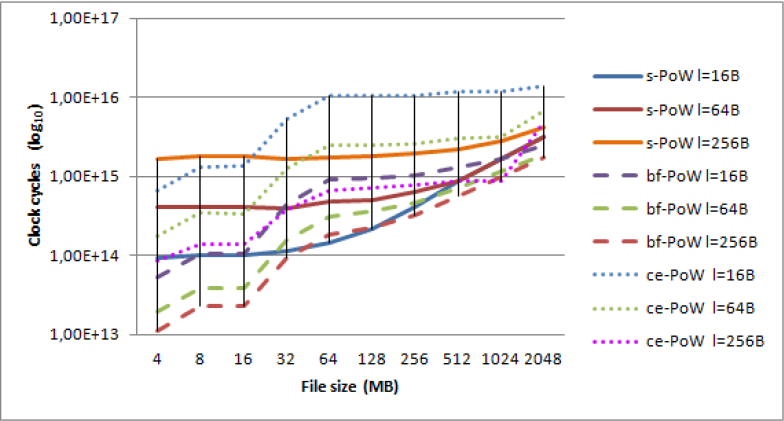
\includegraphics[height=210pt,width=400pt]{ce-POW}
\caption{Comparison of the server side initialization phase: ce-POW, s-POW and bf-POW \cite{ce-POW}}
\label{fig:ce-POW} .
\end{center}
\end{figure}

On the client side the picture is the same bf-POW is the fastest solution while the s-POW is the slowest. The ce-POW is much beater then s-POW solution and is comparison with bf-POW, but again it is important to see that only the ce-POW addresses the privacy and confidentiality issues fro both client and server side.


\subsection{Summary}
\label{subsub:ApproachSummary}

The section \hyperref[sec:4]{Approach} covered the seven different solutions, which addresses the privacy and the confidential issues in remote storage during the data deduplication. It is fundamental to understand in details  the \hyperref[sub:Soltuion1]{state-of-art solution}, also refereed as PoW introduced by Halevi. He addresses the cause of the problem (using the hash-as-a-proxy) and offers the novel solution to deal with it. All the other solutions covered in previews subsections were inspired by Halevi's work. Some of them(Solutions \hyperref[sub:Soltuion4]{4}, \hyperref[sub:Soltuion4]{5}, \hyperref[sub:Soltuion4]{7}) expend the  attack vectors and implement the mix of encryption and proof of ownership, in order to avoid the servers to profile the data of their users. Most of them improve the security, by avoiding the restriction of choosing the file from the particular class of distribution, which is hard to proof. Detail understanding of how each scheme works and what are their security and efficiency criteria, helps to move on the next section and evaluate them in comparison with each other.  

%Outlines the main thing your thesis does. Your thesis describes a novel algorith for X? Your main contribution is a case study that replicates Y? Describe it here.
\pagebreak

%------------------------------EVALUATION-----------------------------------
\section{Evaluation}
\label{sec:5}
Previews section had covered the details of the existing solutions for proof of data ownership in remote storage during the data deduplication. Implementing of those solutions and evaluate there efficiency in terms of I/O and CPU performance is out of scope of this work. Instead this section address bandwidth and space consumption, which could be calculated without implementation of the solutions. Based on the results, we can see addition cost that should be payed to maintain the security level. Calculation is  based on the AWS prices. \footnote{\url{https://aws.amazon.com/s3/pricing/}}. But before the cost analyses, we cover the security aspects of the schemes and evaluates them based on their characteristics described in previews sections.

\subsection{Security Evaluation}
\label{sub:SecurityEva}
It is not straightforward to compare the security of the provide solutions. In the most cases the probability of breaking the security of the scheme is negligible in the given security parameter $k$ and $k$ is always tunable. But the diversity follows from the differences of the attacks that the schemes are addressing and also from the restrictions  in security definition of the protocols. We have demonstrated five general type of attacks in previews sections: File Detection (the adversary uploads the file and observers, whether the deduplication occurs or not), Content Detection (brute-forcing  the content of the file with low min-entropy, detection via deduplication),CDN (using the remote storage as a Content Distribution
Network, while it is not meat to be the one),  Honest-but-curios-servers(Servers are able to access the private data of the user as it is available in clear text) and Poison Attack (When encrypted file is uploaded on server side, server is not able to check consistency between file and meta-data (e.g. hash of the file)). In the \hyperref[table:Attacks]{table} below is demonstrated which solutions address to which particular attacks.\\\\
\begin{savenotes}
\begin{table}[!htpb]
\centering
\addtolength{\tabcolsep}{3pt}
\begin{tabular}{|L{3.5cm}|C{2.5cm}|C{2.1cm}|C{1.5cm}|C{2.5cm}|C{2.5cm}|}
\rowcolor{lightblue}
\hline
&File Detection&Content Detection&CDN&Honest-but-curios-servers&Poison Attack\\ \hline
\hyperref[sub:Soltuion1]{Solution 1} PoW&\checkmark&\checkmark&\checkmark&--&N/A\footnote{the scheme does not uses convergent encryption and the Poison Attack is not applicable.} \\ \hline

\hyperref[sub:Soltuion2]{Solution 2} s-POW&\checkmark&\checkmark&\checkmark&--&N/A\\ \hline

\hyperref[sub:Soltuion3]{Solution 3} POF&\checkmark&\checkmark&N/A&--&N/A\\ \hline

\hyperref[sub:Soltuion4]{Solution 4} {CSD}&\checkmark&\checkmark&\checkmark\ &\checkmark&\checkmark \\ \hline 
%it restricts the data leakage size and security holds if the leakage takes place only before the protocol starts, while in PoW leakage could happen any time, but not the during protocol communication.

\hyperref[sub:Soltuion5]{Solution 5} OpenStack based&\checkmark&\checkmark&\checkmark&\checkmark&\checkmark\\ \hline

\hyperref[sub:Soltuion6]{Solution 6} bf-POW&\checkmark&\checkmark&\checkmark&--&N/A\\ \hline

\hyperref[sub:Soltuion7]{Solution 7} ce-POW&\checkmark&\checkmark&\checkmark&\checkmark&\checkmark \\ \hline
\end{tabular}
\caption{Comparison:  Attacks }
\label{table:Attacks}
\end{table}
\end{savenotes}
\noindent Under the security of the scheme/protocol, we imply the probability of the adversary to pass the protocol and convince the verifier. The lower the probability is , more secure is the scheme. In most cases it is demonstrate that the probability of success is negligible in security parameter. To demonstrate the soundness of their schemes authors use different approaches. The \hyperref[sub:Soltuion1] {Solution 1 - PoW} uses simluation-based approach, and claims that the scheme is secure with soundness  $\left( \frac{L-d+1}{L}\right)^t$ where $L$ is reduce buffer, $t$ is number of challenges on Merkle-tree and $d$ is the minimum distance of the linear code. The variables $L,d\ and\ t$, all are tunable and leads to the negligible probability of adversary's success to convince the verifier. The \hyperref[sub:Soltuion2] {Solution 2 - s-PoW}, also uses  simulation-based approach and demonstrates the negligible probability of adversary to cheat the verifier. $P(succ) = (1-\varepsilon(1-g))^K$, where $\varepsilon$ is a fraction of the file that is unknown for attacker and $g$ is the probability to guess unknown bit correctly and $K$ is the length of response bit string. It is possibility to choose $K$ (depends on security parameter), in such a way that the $P(succ)$ became negligible in security parameter. Security analyses in \hyperref[sub:Soltuion3]{Soltuion 3 - POF} is superficial. The scheme  provides the proof that the cheating of the scheme is at least as hard as "performing strong collision attack of the hash function". And the probability of collision attack is calculated based on Birthday Paradox\footnote{"Given k randomly generated values, where each value is a non-negative integer less than N, what is the probability that at least two of them are equal?" \url{http://preshing.com/20110504/hash-collision-probabilities/} last seen October 3, 2016}. The probability of collision $P=1- \epsilon^{\frac{-k(k-1)}{2N}}$, where $k$ is number of inputs and $N$ is a number of all possible hash values(outputs).(e.g for SHA-256 probability of collision $p=\epsilon^{\frac{-k(k-1)}{2* 2^{256}}}\approx\epsilon^{-\frac{k^2}{2* 2^{256}}}\approx\epsilon^{-\frac{1}{2}( \frac{k}{2^{128}})^2}$). The security analyses of the   \hyperref[sub:Soltuion4]{Solution 4 - $CSD$}, differs from other solutions, as it uses the game-based security proof approach. Based on  two players $A$ - adversary and $A_*$ -- extractor, is defined, that the scheme is secure in $(\varepsilon_0, \varepsilon_1)$ if the probability of guessing $b$ single bit by extractor $A_*$ plus some negligible in security parameter $negl(\lambda)$, is grater or equal then probability of adversary $A$ guessing the same $b$ bit: $Pr[b_A=b]\leq Pr[b_{A_*}=b]+negl(\lambda)$.Where $\varepsilon_0$ is a minimum min-entropy of the file and $(\varepsilon_0 - \varepsilon_1 )$ – is a max length of bits adversary is allowed to learn. The security analyses are practically missing(or are provided very briefly) in  \hyperref[sub:Soltuion5]{Solutions 5} and do not covers the probability of success of adversary. The last two solutions both offer the security analyses and demonstrate the probability of adversary convincing the verifier, which are negligible in security parameter and depend in both cases on $J$ -- number of tokens generated by prover as the response on the challenge received from verifier.  For  \hyperref[sub:Soltuion6]{Solution 6 - bf-POW} the probability of success is $(p+(1-p)(0.5^l)+p_f(1-0.5^l))^J$. While for \hyperref[sub:Soltuion7]{Solution 7 - ce-POW} $P(succ) = (p+(1-p)*0.5^l)^J$. Where in both cases $p$ is the probability that adversary knows the randomly chosen chunk, $g$ is the probability to guess the randomly chosen byte, $l$ is a token size and $p_f$ in \hyperref[sub:Soltuion6]{Solution 6} is a probability of false positive in BF.\\\\
Besides the soundness of the scheme, it is significant to underline the leakage resilience  and restrictions of the schemes. The most of the solutions defines a threshold $T$ of data leakage, and if the adversary learns up to $T$ bits, the security of the scheme still holds(e.g.  \hyperref[sub:Soltuion1]{PoW} the threshold is set to $64Mb$). In some solutions the adversary can communicate with accomplices and receive the information up to given threshold, but it should take place before or after the protocol is running. While the last solution (ce-POW)  allows receiving the information about file only before the protocol starts. It is important to underline that in \hyperref[sub:Soltuion1]{PoW}, the files are take from specific class of distributed, while later schemes build there security definition based, on arbitrary file distribution.  The summary of security analyses, is provided in the \hyperref[table:Security]{table} below.

\begin{savenotes}
\begin{table}[!htpb]
\centering
\addtolength{\tabcolsep}{3pt}
\begin{tabular}{|L{3cm}|C{3cm}|C{4cm}|C{5cm}|}
\rowcolor{lightblue}
\hline
&Input File&Leakage Resilience &Soundness\\ \hline
\hyperref[sub:Soltuion1]{Solution 1} PoW&Specific Class of Distribution&\checkmark& $\left( \frac{L-d+1}{L}\right)^t$ \footnote{$L$ is reduce buffer, $t$ is number of challenges on Merkle-tree and $d$ is the minimum distance of the linear code.} \\ \hline
\hyperref[sub:Soltuion2]{Solution 2} s-PoW&Arbitrary Distribution &\checkmark&$P(succ) = (1-\varepsilon(1-g))^K$\footnote{ $\varepsilon$ is a fraction of the file that is unknown for attacker and $g$ is the probability to guess unknown bit correctly and $K$ is the length of response bit string.} \\ \hline
\hyperref[sub:Soltuion3]{Solution 3} POF&N/A&--&Probability of Collision  in  Hash Function\\ \hline
\hyperref[sub:Soltuion4]{Solution 4} {CSD}&Arbitrary Distribution&\checkmark& $Pr[b_A=b]\leq Pr[b_{A_*}=b]+negl(\lambda)$\footnote{.$\varepsilon_0$ is a minimum min-entropy of the file and $(\varepsilon_0 - \varepsilon_1 )$ – is a max length of bits adversary is allowed to learn} \\ \hline
\hyperref[sub:Soltuion5]{Solution 5} OpenStack based&Arbitrary Distribution&N/A&Security Based on Merkle-tree lemma\cite{MerkleLemma} \\ \hline
\hyperref[sub:Soltuion6]{Solution 6} bf-POW&Arbitrary Distribution&\checkmark&$P(succ)=(p+(1-p)(0.5^l)+p_f(1-0.5^l))^J$\footnote{ $p$ is the probability that adversary knows the randomly chosen chunk, $g$ is the probability to guess the randomly chosen byte, $l$ is a token size and $p_f$  is a probability of false positive in BF} \\ \hline
\hyperref[sub:Soltuion7]{Solution 7} ce-POW&Arbitrary Distribution&\checkmark&$P(succ) = (p+(1-p)*0.5^l)^J$\footnote{ $p$ is the probability that adversary knows the randomly chosen chunk, $g$ is the probability to guess the randomly chosen byte, $l$ is a token size} \\ \hline

\end{tabular}
\caption{Comparison:  Security Features }
\label{table:Security}
\end{table}
\end{savenotes}

The results demonstrate that most preferable choices in terms of security are the \hyperref[sub:Soltuion4]{solution 4} and the \hyperref[sub:Soltuion7]{solution 7}. They ensure that the client and the server both are the honest player. Both avoid the file and content detection attacks by implement the proof of ownership, avoid confidential data profiling by implementing  encryption and avoid position attack by implementing additional check over encrypted files. Their security is build on the files taken form arbitrary distribution and allow the predefined amount of data leakage, which prevents from CDN attack. On the other hand less preferable choices are  \hyperref[sub:Soltuion3]{solution 3} and \hyperref[sub:Soltuion5]{Solution 5}. The \hyperref[sub:Soltuion3]{Solution 3}  does not cover the honest-but-curios-server's issue and also the authors do not provide the discussion about leakage resilience in a straightforward manner. There for it is also not clear to measure the tolerance to the CDN attack. As regards to the \hyperref[sub:Soltuion5]{Solution 5} - the paper covers the security analyses of the scheme  superficially and do not provide the probability of success of adversary. It is also hard to calculate the leakage resilience of the scheme. But the solution  addresses the  data privacy issues in the remote storage and uses encryption and Merkle-tree to avoid the cheating form both players(client and server). The drawback of \hyperref[sub:Soltuion2]{Solution 2} and \hyperref[sub:Soltuion6]{Solution 6} is that they consider the server as a honest player and does not ensure the client data privacy. But both of them have the clear image of the probability of success of adversary to cheat the scheme and it is calculated based on arbitrary distributed files in both cases. Disadvantaged of the first solution-\hyperref[sub:Soltuion1] {PoW} is that it builds the security on the assumption that the files are taken form the specific distribution class and it is hard to proof such assumption. Also it does not address the honest-but-cures-server's issues.


\subsection{Cost Analyses}
\label{sub:Cost}

The aim of the data deduplication is the reduction of bandwidth and disk space consumption. All the solutions covered above, carries the extra calculation in order to maintain the security. It increases  the bandwidth and storage consumption in comparison with not secure "hash-as-a-proxy" solution. But those seven solutions still are more efficient then "whole file transfer" approach. This section evaluates the additional  generated data traffic and disk space for each scheme, and  calculates the cost  based on the Amazon S3 Pricing.\footnote{\url{https://aws.amazon.com/s3/pricing/}, last seen October 3, 2016}\\\\
In the \hyperref[sub:Soltuion1]{Solution 1} -- PoW, the server asks for the  randomly chosen $20$ leaves  and their sibling paths of the Merkle-tree. Sibling path consists of the sibling node of the given leaf and also all the parent sibling nodes values, from the sibling leaf till the roof of the tree. So the client generates the sibling path $P=(v_s,v_{n_0},v_{n_1},...,v_{n_i})$, where $v_s$ is a value of the sibling node \footnote{The value of the node of the Merkle-tree is the corresponding block if the node is a leaf or the hash of the left and right children if it is an intermediate node.}, $i$ is the hight of the Merkle-tree and $v_{n_0},v_{n_1},...,v_{n_i}$ are the values of the parent nodes. The maximum buffer size is $64MB$. The leaf size is $256$ bits. So in worst case the Merkle tree has $\frac{64 * 1024* 1024 * 8}{256} = \frac{2^6*2^10*2^10*2^3}{2^8}=2^{21}$ leafs and the height of tree is 21.The size of sibling path is $2*21*256=10752$ bits  $\approx 1.3 KB$. The traffic generated by PoW is $20$ times sibling path size, which is approximately $\color{blue}26KB$ "Data Transfer In" operation for remote storage. As regards to the extra disk space consumption, the server requires to store the root value (plus number of leaves, which is negligible size) -- output of hash function, $\color{blue}256\ bits$  long string (hash function used in implementation is SHA256).\\\\
 For the \hyperref[sub:Soltuion2]{Solution 2} -- s-POW -- generated traffic includes: the random seed $s$, which server sends to the client and the client's response: $K$ bits long string called $response$. $s$ is an integer $0<s<file\_size$, so it is negligible($4$ bytes), and the response length is tunable, the maximum size used in paper is $1830$ bits. The traffic generated during the proof is  approximately $\color{blue}0.23 KB$. To look at the space consumption, for each file it is a tuple the server keeps in the database. The tuple contains  $4$ elements: $ptr$ -- the pointer on the file --$8$ byte long. $res []$ -- an $10000$ length array of generated challenges, called "responses" -- each for $1830$ bits length string; $id_c$ -- the highest challenge computed so far -- integer $2$ bytes; $id_u$ -- number of challenges used so far-- integer $2$ bytes and finally it uses the hash of the file as a key. The following formula calculates total extra space: $256$ bits (hash of file) + $64$ bits(ptr) + $10 000 * 1830$ bits(array) + $32$ bits ($id_c$) + $32$ bits ($id_u$) = $18300384$ bits $\approx\color{blue}2.29MB$. \\\\  
 During the POF protocol in the \hyperref[sub:Soltuion3]{Solution 3}, the client and the server  exchange the following data: The hash value of file $h(F)$ (hash function is SHA256) ; $R_c$ the random number $R_c \leftarrow _R \{0,1\}^*$ -- for calculation consider the length of the $R_c$ to be $256$ bits; Two random seeds -- $S_1 \leftarrow _R \{0,1\}^*$ and 
 $S_2 \leftarrow _R \{0,1\}^*$ -- consider them as $256$ bits long;  The integer $c$ -- number of blocks -- 32 bits long; Client confirmation of obtaining the session key $h_{K_s}(R_c,TS)||TS$ -- concatenation of hash value and TimeStamp -- output of SHA256 plus the value of unix Timetamp($32$ bit length); And finally the summary value, the proof-- hash of concatenation of hashes of chosen blocks -- $256$ bits long (again using the SHA256). To sum up the generated data, we will have a following result: total data transfer In =  $256$ bits (hash of file) +
 $256$ bits (hash of $R_c$ with session key) + $32$ bits(TimeStamp)+ $256$ bits (the proof) = $\color{blue} 100\ Bytes$ and total data transfer Out = $32$ bits ($c$ number of blocks) + $256$ bits ($R_c$) + $2*256$ bits ($S_1$ and $S_2$) = $\color{blue} 80\ Bytes$. The \hyperref[sub:Soltuion3]{solution 3} generates in total approximately $0.1 KB$ traffic, which is very efficient. And the protocol is even more efficient in terms of the disk space consumption, it occupies only extra $\color{blue}256\ bits$ (hash value of file) per file same as "hash-as-a-proxy" solution.\\\\
The \hyperref[sub:Soltuion4]{Solution 4} adds encryption over the proof of ownership protocol and generates the following traffic: The client sends the hash of the file $hash(F)$ to the server - $256$ bits string. The server challenges the client and sends back the encrypted AES key $C_\tau$-- less then $256$  bits length string. To proof the ownership of the file the client  sends the hash value of AES encrypted file -- also the size is $256$  bits. The generated traffic per file is totaling to:$2*256=512\ bits=\color{blue}64\ Bytes$ for data transfer In and $\color{blue}32\ Bytes$ - data transfer Out. Disk space required for protocol consists of the encrypted file and the meta-data. The size of encrypted file is approximately same as the plain file.\footnote{The AES-256 output calculation: $CipherText_{size} = PlainText_{size} + Block_{size(256)} - (PlainText_{size}\ MOD\ Block_{size(256)})$}  And the size of meta-data is the size of the following key-value pair: $(key = hash(F); value = (hash(C_F), C_\tau))$. Total  $256$ bits ($hash(F)$) + $256$ bits($hash(C_F)$) + $256$ bits($C_\tau$) $\approx0.1KB$. The additional storage is $\approx\color{blue}0.1KB$.\\\\
Data exchange between the client and the server in the \hyperref[sub:Soltuion5]{Solution 5} looks as  following: the client first sends the Merkle-tree root value over the encrypted file to the server  -- 256 bits string. The server request the super-logarithmic number of leaves and the sibling paths, same as the \hyperref[sub:Soltuion1]{Solution 1} scenario , meaning the  approximately $\color{blue}26KB$ data transfer In. And if the proof holds then the server sends the URI of the requested file. Swift restriction -- length of container is maximum $256$ bytes and the maximum length of object name is $1024$ bytes.\footnote{\url{http://docs.openstack.org/developer/swift/api/object_api_v1_overview.html}, last seen October 3, 2016} Hence the generated data transfer Out is $\color{blue} 1280\ Bytes$. As for extra disc space -- it is only $\color{blue}256\ bits$  long and represents the Merkle-tree root value of encrypted file.\\\\
In \hyperref[sub:Soltuion6]{Solution 6} the bandwidth  and storage consumption, both are depending on token size. If token size is small -- bandwidth consumption is low, while the required disk space grows. The growth of tokens size cause the growth of data traffic, but the  decrease  of storage consumption. In worst case scenario the extra storage consumption is $\color{blue}2MB=2000KB$ for the tokens $128$ bits length, but it could be decreased to $\color{blue}40\ bytes=0.04KB$ . In order to prove the ownership the following data is generated: $256$ bits (the hash of the file)  +  $J\ *\ 32 $ bits ( the $J$ length array( $pos []$) of the integers)+ $J\ *\ 1024$ bits (the $J$ length array($res[]$) of $tokens$(max length of token size in paper is $1024$ bits) = $256$ bits + $1040*J$ bits. Where $J \in \{102,\ 204,\ 509,\ 1017\}$. Taking into consideration a worst case scenario, the generated data during the bf-POW protocol is $256 + 1024*1017 = 1041664\ bites\approx \color{blue}130KB$ In and $32*1024=32768\ bites\approx \color{blue}4KB $ Out data transfer, while it could be decreased till $256+128*102=13312\ bites\approx\color{blue}1.7KB$ In and $32*128= \color{blue}512\ Bytes$ Out data transfer.\\\\
The last solution \hyperref[sub:Soltuion7]{Solution 7} is similar to the \hyperref[sub:Soltuion6]{Solution 6} in terms of bandwidth consumption. First client sends the file identifier -- output of SHA-1 160 bits. Then server challenges the client and sends the $J$ length $pos[]$ array of integers -- $J\ *\ 32$ bits. In response the client  sends back to the server the $J$ length array $res[]$ of $tokens$(max length of token size in paper is $1024$ bits). And the  $J \in \{91,\ 182,\ 457,\ 914\}$. In worst case scenario the ce-POW protocol generates $160+914*32\approx \color{blue} 3.6 KB$ data transfer Out and  $1024*914+160=\approx \color{blue} 117 KB$ data transfer In. The additional disk space required for protocol is the sum of the identifier (output of SHA1 -- 160 bits), $10 000$ length array of $J$ numbers($10000*914$ bits) and same length array of pre-calculated responses ($10000*914*1024$ bits).Total = $160 + 10000*914(1+1024)=9368500160$ bits $\approx \color{blue} 1.1 GB $.\\\\
In order to demonstrate the extra cost of the solutions, the \hyperref[table:AWS-S3]{table} contains the calculation using the Amazons S3 - simple monthly calculator \footnote{\url{https://calculator.s3.amazonaws.com/index.html} last seen September 29, 2016}. To have an approximate  picture of  volume of the average remote storage providers, I have refereed to the statistics of one of the most popular storage provider -- Dropbox.\footnote{\url{http://expandedramblings.com/index.php/dropbox-statistics/}, last seen September 29, 2016 }.
The numbers are impressive, Dropbox daily receives 1.2 billion files and by the year of 2015, it was storing 35 billion Microsoft Office files. Taking into consideration also the deduplication ration -- $4:1$\footnote{\url{https://www.ibm.com/developerworks/community/wikis/home?lang=en\#!/wiki/Tivoli+Storage+Manager/page/Deduplication+FAQ} last seen September 29, 2016}  (this is an average ratio, when the nature of data is unknown) we can assume that the remote storage provider could duplicate daily $\frac{1200 000 000}{\frac{3}{4}}=900000000$ files -- 30 monthly, and store more the 35 Billion files.( As 35 billion is the number of only Microsoft office files and the user's content is much more reach then just the office files)
%   ${\scriptstyle\href{}{\textit{see the monthly bill}} }$

\begin{savenotes}
\begin{table}[!htpb]
\centering
\addtolength{\tabcolsep}{3pt}
\begin{tabular}{|L{3cm}|L{4.7cm}|L{4.5cm}|L{3.5cm}|}
\rowcolor{lightblue}
\hline
&Traffic&Storage&Total Cost \\
\hline
{\small\hyperref[sub:Soltuion1]{Solution 1}}&${\scriptstyle26KB\ *\ 9*10^8 =\ 23.4TB (In) }$&${\scriptstyle256\ Bits\ * \ 35*10^9\ =\ 1.12TB}$& ${\scriptstyle\$\ 34.2\  \href{https://calculator.s3.amazonaws.com/index.html\#key=calc-965FEE16-BA20-4E18-859A-E7C9B0C0642F}{\textit{see the monthly bill}}}$\\
\hline
{\small\hyperref[sub:Soltuion2]{Solution 2}}&${\scriptstyle0.23 KB \ *\ 9*10^8\ =\ 193GB(In)}$&${\scriptstyle2.29 MB\ * \ 35*10^9\ =\ 80.15PB}$&${\scriptstyle\$ \ 2390882.94 \ \ \ \href{
https://calculator.s3.amazonaws.com/index.html#r=IAD&s=S3&key=calc-EBD5E29A-89DA-489E-8D03-1278B9B3868D}{\textit{see details }} }$\\
\hline
{\small\hyperref[sub:Soltuion3]{Solution 3}}&${\scriptstyle 100\ Bytes\ *\  9*10^8 = 90GB(In)}$  ${\scriptstyle 80\ Bytes\ *\ 9*10^8 = 72GB(Out)}$&${\scriptstyle256\ Bits\ *  \ 35*10^9\ =\ 1.12TB}$&${\scriptstyle \$\ 39.33\  \href{https://calculator.s3.amazonaws.com/index.html\#r=IAD&s=S3&key=calc-09D057D3-F7C4-451A-8A8B-A809B8823C21}{\textit{see the monthly bill}} }$\\
\hline
{\small\hyperref[sub:Soltuion4]{Solution 4}}&${\scriptstyle 64\ Bytes\ *\ 9*10^8\ =\ 57.6GB(In)}$  ${\scriptstyle 32\ Bytes\ *\ 9*10^8\ =\ 28.8GB(Out)}$&${\scriptstyle0.1 KB\ * \ 35*10^9 =\ 3.5TB}$&${\scriptstyle\$\ 107.34\  \href{https://calculator.s3.amazonaws.com/index.html\#key=calc-86396F9E-A16F-4F71-BF27-AC06643F652F}{\textit{see the monthly bill}} }$\\
\hline
{\small\hyperref[sub:Soltuion5]{Solution 5}}&${\scriptstyle 26KB\ *\ 9*10^8\ =\ 23.4TB (In)}$  ${\scriptstyle 1280\ Bytes\ *\ 9*10^8\ =\ 1.15TB(Out)}$&${\scriptstyle256\ Bits\ * \ 35*10^9\ =\ 1.12TB}$&${\scriptstyle\$\ 128.84\ \href{https://calculator.s3.amazonaws.com/index.html\#r=IAD&s=S3&key=calc-1FCB17FA-8FF2-417E-B0EF-0961F732045A}{\textit{see the monthly bill}} }$\\
\hline
{\small\hyperref[sub:Soltuion6]{Solution 6}}&${\scriptstyle\ \ \ 130KB\ *\ 9*10^8\ =\ 117TB(In)}$ ${\scriptstyle\ \ \ 4KB\ *\ 9*10^8\ =\ 3.6TB(Out)\ \ \ }$ or ${\scriptstyle\ \ \ 1.7KB\ *\ 9*10^8\ =\ 1.5TB(In)\ \ \ }$  ${\scriptstyle\ \ \ 512 Bytes\ *\ 9*10^8\ = \ 430GB(Out)}$ &${\scriptstyle\ \ \ 1.7 KB\ * \ 35*10^9 =\ 59.5TB\ \ \ }$ or ${\scriptstyle\ \ \ 132 KB\ * \ 35*10^9 =\ 4.62PB\ \ \ }$&${\scriptstyle\ \ \ \$\ 2335.65\ \href{https://calculator.s3.amazonaws.com/index.html\#r=IAD&s=S3&key=calc-21352AB8-9DB2-42E4-98A1-520A2A0D9074}{\textit{see details}} \ \ \ \ \ \ }$ or ${\scriptstyle\ \ \ \$ \ 145198.87\ \href{https://calculator.s3.amazonaws.com/index.html\#r=IAD&s=S3&key=calc-F542BEAC-D18B-48CB-876F-B5FD926FD93E}{\textit{see details}}\ \ \ \  }$\\
\hline
{\small\hyperref[sub:Soltuion7]{Solution 7}}&${\scriptstyle 117KB\ *\ 9*10^8\ =\ 105.3TB(IN)}$  ${\scriptstyle 3.6 KB\ *\ 9*10^8\ =\ 3.24TB(Out)}$& ${\scriptstyle1.1 GB \ *\ 35*10^9=\ 38500PB}$&${\scriptstyle\$\ 1143495895.96\ \href{https://calculator.s3.amazonaws.com/index.html\#r=IAD&s=S3&key=calc-0F562F39-A8CB-4A30-93EE-614F360CC1ED}{\textit{see details}} }$\\
\rowcolor{gray}
\hline
{\small"Hash-as-a-proxy"}&${\scriptstyle 32\ Bytes\ *\ 9*10^8\ =\ 28.8GB(In) }$&${\scriptstyle256\ Bits\ *  \ 35*10^9\ =\ 1.12TB}$&${\scriptstyle \$\ 34.2\ \href{https://calculator.s3.amazonaws.com/index.html\#r=IAD&s=S3&key=calc-827C7B47-F08D-4275-8F06-38845EB73750}{\textit{see the monthly bill}} }$\\

\hline

\end{tabular}
\caption{Data traffic and storage costs based on Amazon S3 pricing. Estimated amount of files and generated traffic is offered  according the static of one of the most popular remote storage provider - Dropbox.}
\label{table:AWS-S3}
\end{table}
\end{savenotes}

In terms of the cost  we can see from the \hyperref[table:AWS-S3]{table} that most efficient is \hyperref[sub:Soltuion1]{Solution 1} - PoW, which has the same  expense as the non secure "Hash-as-a-proxy" solution. After comes  \hyperref[sub:Soltuion3]{Solution 3}, with \$\ $39.33$ in month. Third and fourth places are respectively for  \hyperref[sub:Soltuion4]{Solution 4} and  \hyperref[sub:Soltuion5]{Solution 5}. The \hyperref[sub:Soltuion6]{Solution 6} is on fifth position with \$\ $2335.65$ per month and  after come the  \hyperref[sub:Soltuion2]{Solution 2} and  \hyperref[sub:Soltuion7]{Solution 7} where the price dramatically grows and is practically not affordable. 

%\begin{tikzpicture}
%\begin{axis}[
%legend columns=-1,
%legend cell align=left,
%every axis plot post/.style={/pgf/number format/fixed},
%ybar=2pt,
%bar width=10pt,
%x=5cm,
%y=4.5cm,
%ymin=0,
%axis on top,
%ymax=12,
%xtick=data,
%xlabel=Cores,
%ylabel=Cost in Bilions USD,
%enlarge x limits=0.2,
%enlarge y limits={abs=0.5},
%symbolic x coords={Solutions,Beta pi},
%restrict y to domain*=0:11, % Cut values off at 14
%visualization depends on=rawy\as\rawy, % Save the unclipped values
%after end axis/.code={ % Draw line indicating break
%\draw [ultra thick, white] (rel axis cs:0,1.05) -- (rel axis cs:1,1.05);
%    },
%nodes near coords={\scriptsize{\pgfmathprintnumber{\rawy}}
%    },
%axis lines*=left,
%clip=false,
%area legend
%legend style={at={(0.6,0.8)},anchor=west}
%]
%\addplot[fill=red!40] coordinates {(Solutions,0.000000034)  };
%\addplot[fill=yellow!40] coordinates {(Solutions,1)  };
%\addplot[fill=blue!40] coordinates {(Solutions,0.6) };
%\addplot[fill=green!40] coordinates {(Solutions,1.14) };
%\legend{x264,bodytrack,swaptions,blacksholes};
%\end{axis}
%\end{tikzpicture}



%\subsection{Efficiency Evaluation}
%\label{sub:EfficiencyEva}
%The security aspects of the solutions is dominant, while choosing the scheme for implementation. But in real life scenarios the efficiency of the scheme influence the decision and in some %cases determines the choice. Implementation and execution of the solutions, in order to evaluate their performance is out of the scope of this work. The subsection compares the performance %of the solution based on the efficiency analyses provided by the authors of the papers. Some of the solution provide the asymmetric analyses, we can merge them in the %\hyperref[table:asymptoticAnal]{table} bellow and have bigger picture.  
%\begin{savenotes}
%\begin{table}[!htpb]
%\centering
%\addtolength{\tabcolsep}{3pt}
%\begin{tabular}{|L{3cm}|L{2.5cm}|L{2.5cm}|L{3.5cm}|L{2.5cm}|}
%\rowcolor{lightblue}
%\hline
%&PoW&s-POW&bf-POW&ce-POW\\
%\hline
%Client computation&$O(F)hash$ & $O(F)hash$ & $O(F)hash$&$O(B)*CE*hash*hash$  \\
%\hline
%Client I/O&$O(F)$&$O(F)$&$O(F)$&$O(F)$\\
%\hline
%Server init computation &$O(F) hash$&$O(F) hash$&$O(F)hash$&$O(B)*hash*hash$\\
%\hline
%Server regular computation &$O(1)$&$O(nk) PRF$& $O(\frac{l*k*(log1/p_f)}{p_f})hash$&$O(n * l *k)*PRNG$\\
%\hline
%Server init I/O &$O(F)$&$O(F)$&$O(F)$&$O(F)$\\
%\hline
%Server regular I/O &$O(0)$&$O(nk)$&$O(0)$&$O(0)$\\
%\hline
%Server memory usage&$O(1)$&$O(nk)$&$O(\frac{log(1/p_f)}{l})$\\
%\hline
%Bandwidth&$O(k\ log\ k)$&$O(k)$&$O(\frac{lk}{p_f})$\\
%\hline

%\end{tabular}
%\caption{Asymptotic analyses of schemes. $F$ is the file size; $B$ is a chunk size; $k$ is a security parameter; $n$ is number of challenges in s-POW;  $l$ is a $PRF$ output size; $p_f$ is %a probability of false positive in BF}
%\label{table:asymptoticAnal}
%\end{table}
%\end{savenotes}
%Time efficiency analyses provided by authors, are decomposed in three parts: client side , server side and network efficiency. This subsection covers the client and server side efficiency, %while the next section covers network related part. To demonstrate the efficiency of their schemes authors implement together with their own scheme, other solution and make the comparison. The \hyperref[sub:Soltuion1]{Solution 1} - PoW is compared with the "using-hash-as-a-proxy"(non secure solution) and "transferring the whole file" solutions. The server side effort in PoW protocol is negligible, as it checks the Merkle-tree signature based on provided leaves and sibling paths(In the paper the requested leaves number is set to 20 and the server  spend $0.6ms$ on the signature check.).On the other hand, in whole file transfer approacher there is no checking operation at all, but this approach has the drawback in terms of bandwidth and space efficiency. The "hash-as-a-proxy" approach performs is only look up operation on server side, which is more efficient then checking the Merkle-tree signature, but also this solution hash the drawback in terms of security. PoW is also compared with the \hyperref[sub:Soltuion2] {Solution 2} - s-POW and on server side it was demonstrated that PoW--Merkle-Tree signature verification is more efficient then s-POW, lookup operation plus recalculate of the "challenges" which are stored in "res[]" array. The \hyperref[sub:Soltuion3]{Solution 3} on server side  generates session key, random seeds, random indices , dynamic coefficients  and $\tau+1$ hash operation, where $\tau$ is a number of random blocks. It is also compared with \hyperref[sub:Soltuion1]{Solution 1} and on the server side the first solution is again more efficient the POF. While the \hyperref[sub:Soltuion4] {Solution 4} does not covers details of performance of the scheme it is not decomposed on server side and client side performance evaluation and provides only the comparison  with "whole file transfer" approach in \hyperref[fig:POWvsPoW]{graph}. Similar comparison has provided PoW in its \hyperref[gif:PoWgraph]{graph}. We can compare those two solution with a little inaccuracy (as they are not run on the same platform) to each other for 5Mbps network implementation.

%From the \hyperref[fig:POWvsPoW]{graph} we can see that the \hyperref[sub:Soltuion4] {Solution 4} is faster. We still can compare it with \hyperref[sub:Soltuion1] {Solution 1} PoW protocol, as both are align with "whole file transfer" solution. We can compare with a small inaccuracy (as they are not run on the same platform), the those two solutions performance, for network $5Mbps$ and file size $128, 256, 512\ and\ 1024$ MB.


%In \hyperref[sub:Soltuion1] {PoW} 
%is an integer less or equle the number of blocks   and on server side again the PoW is more efficient then POF
%as it includes recalculate of the challenges


\subsection{Summary}
\label{sub:SummeryEva}

The section \hyperref[sec:5]{Evaluation} compared the security characteristics and additional costs for required bandwidth and storage of the solutions. We have identified the most preferable solution from the security point of view and they are: \hyperref[sub:Soltuion4]{Solution 4} and \hyperref[sub:Soltuion7]{Solution 7}. As the \hyperref[sub:Soltuion7]{Solution 7} is no affordable and the cost of the \hyperref[sub:Soltuion4]{Solution 4} is quite realistic -- \$\ 107.34 per month, we can see that the  \hyperref[sub:Soltuion4]{Solution 4} is the optimal choice for implementation. But if the Hones-but-curios servers  is not an issue then it is better to choose the \hyperref[sub:Soltuion1]{Solution 1} as it has the lowest cost. Despite the low cost still not preferable choices are the \hyperref[sub:Soltuion3]{Solution 3} and the \hyperref[sub:Soltuion5]{Solution 5} because of their security \hyperref[table:Security]{characteristics}. Choosing the \hyperref[sub:Soltuion6]{Solution 6} is also not reasonable, because it has the same security features  as the first solutions, in difference that the input files are taken from arbitrary distribution, but the cost is $68$ times more. In most cases the decision which solution to choose depends on implementation's objectives, but in any case solutions \hyperref[sub:Soltuion2]{2}, \hyperref[sub:Soltuion6]{6} and \hyperref[sub:Soltuion7]{7} are out of the game, because of extremely high cost.\\\\ 
In real life scenario to take a decision, it is also important to have the results of I/O and CPU efficiency.  To obtain the result, it is required to implement all the solution in same environment, which is out of scope of this work.




%Describes why your approach really solves the problem it claims to solve. You implemented a novel algorithm for X? 
%This chapter describes how you ran it on a dataset and reports the results you measured. You replicated a study? This chapter gives the results and your interpretations.
%The Appraoch and Evaluation chapters contain the meat of your thesis. Often, they make up half or more of the pages of the entire document.

\pagebreak

%------------------------------FUTURE WORK-----------------------------------
%\section{Future Work}
%\label{sec:6}

% In science folklore, the merit of a research question is compounded by the number of interesting follow-up research questions it raises. 
% So to show the merit of the problem you worked on, you list these questions here.
 %If you don’t care about research folklore (I did not as a student),
 %this chapter is still useful: whenever you stumble across something that you should do if you had unlimited time, but cannot do since you don’t, you describe it here. 
 %Typical candidates are evaluation on more study objects, investigation of potential threats to validity, … 
 %The point here is to inform the reader (and your supervisor) that you were aware of these limitatons. Limit this chapter to very few pages. 
 %Two is entirely fine, even for a Master’s thesis.
%\pagebreak


%------------------------------CONCLUSIONS-----------------------------------
\section{Conclusions}
\label{sec:7}
Short summary of the contribution and its implications. The goal is to drive home the result of your thesis.
Do not repeat all the stuff you have written in other parts of the thesis in detail. Again, limit this chapter to very few pages. 
The shorter, the easier it is to keep consistent with the parts it summarizes.

\pagebreak

%------------------------------REFERENCES-----------------------------------

\addcontentsline{toc}{section}{References}


\bibliographystyle{IEEEtran}
\bibliography{bibi.bib}


\pagebreak

%-----------------------------APPENDIX--------------------------------

\appendix

\section{Appendix 1}

\label{Appendix 1}

\subsection*{POF -- PERFORMANCE MEASUREMENTS AND COMPARISON}



\begin{savenotes}
\begin{table}[!htpb]
\centering
\addtolength{\tabcolsep}{3pt}
\begin{tabular}{|L{2cm}|L{2cm}|L{2cm}|L{2cm}|L{2cm}|L{2cm}|L{2cm}|}
\rowcolor{lightblue}
\hline

&\multicolumn{3}{|C{6.5cm}}{ PoW (ms)}&\multicolumn{3}{|C{6.5cm}|}{POF (ms)}\\ \hline


Size (MB)&Disk Read&Merkle Tree&Total&Disk Read&Algorithm&Total\\ \hline

0.015625&0.09&0.57&0.66&0.15&0.62&0.77 \\ \hline
0.03125&0.13&1.07&1.2&0.16&0.42&0.58 \\ \hline
0.0625&0.19&1.73&1.92&0.17&0.62&0.79 \\ \hline
0.125&0.34&4.01&4.35&0.2&0.63&0.83 \\ \hline
0.25&0.62&6.82&7.44&0.24&0.63&0.87 \\ \hline
0.5&1.17&12.51&13.68&0.27&0.58&0.85 \\ \hline
1&2.03&21.08&23.11&0.29&0.62&0.91 \\ \hline
2&4.44&42.46&46.9&0.31&0.62&0.93 \\ \hline
4&8.19&84.46&92.65&0.55&0.63&1.18 \\ \hline
8&14.76&168.43&183.19&0.66&0.65&1.31 \\ \hline
16&28.62&334.88&363.5&0.82&0.64&1.46 \\ \hline
32&56.75&669.38&726.13&1.32&0.67&1.99 \\ \hline
64&112.58&1352.01&1464.59&4.34&0.64&4.98 \\ \hline
128&223.08&2692.07&2915.15&5.56&0.65&6.21 \\ \hline
256&437.84&5393.64&5831.48&2.11&0.65&2.76 \\ \hline
512&1269.46&10932.49&12201.95&5.53&0.64&6.17 \\ \hline
1024&2581.56&23344.83&25926.39&5.52&0.63&6.15 \\ \hline


\end{tabular}
\caption{Client Computation Time -- POF vs PoW }
\label{table:asymptoticAnalysis}
\end{table}
\end{savenotes}


\end{document}
